% change according to folder and file names
\ifpdf
    \graphicspath{{5/figures/PNG/}{5/figures/PDF/}{4/figures/}}
\else
    \graphicspath{{5/figures/EPS/}{5/figures/}}
\fi

%: ----------------------- contents from here ------------------------
\chapter{Optimization of Hydraulic Turbomachines} % top level followed by section, subsection
%\begin{flushright}
%%Water is for turbines.   
%The Wise Find Pleasure in Water
%\linebreak
%Confucius
%\linebreak
%\end{flushright}

In this chapter, the KBD method presented in Chapter \ref{KBDchapter} and the MAEAs which are further driven by the principal component analysis (PCA) of promising individuals, presented in Chapter \ref{VarCorrChapter}, are used to solve large scale industrial problems related to the design-optimizations  of hydraulic turbines. 

In order to perform a successful optimization, a reliable evaluation procedure must be available. The evaluation procedure used in this chapter (fig. \ref{evaltool}) comprises three parts: the parameterization tool which is able to generate 3D turbine blade shapes, the grid generation tool able to automatically generate computational grids in any geometry created according to the aforementioned paremeterization tool and the CFD software. Section \ref{ParamEval} presents the basic features of the aforementioned tools. Section \ref{Paramt} is about the  parameterization  which is appropriate for 3D geometries of any type of reaction turbines. The grid generation is presented in section \ref{SpaceDisct}. And, finally, the Euler solver used to predict the water flow through the flow passage is presented in section \ref{FlowSolvert}.

\begin{figure}[h!]
\centering
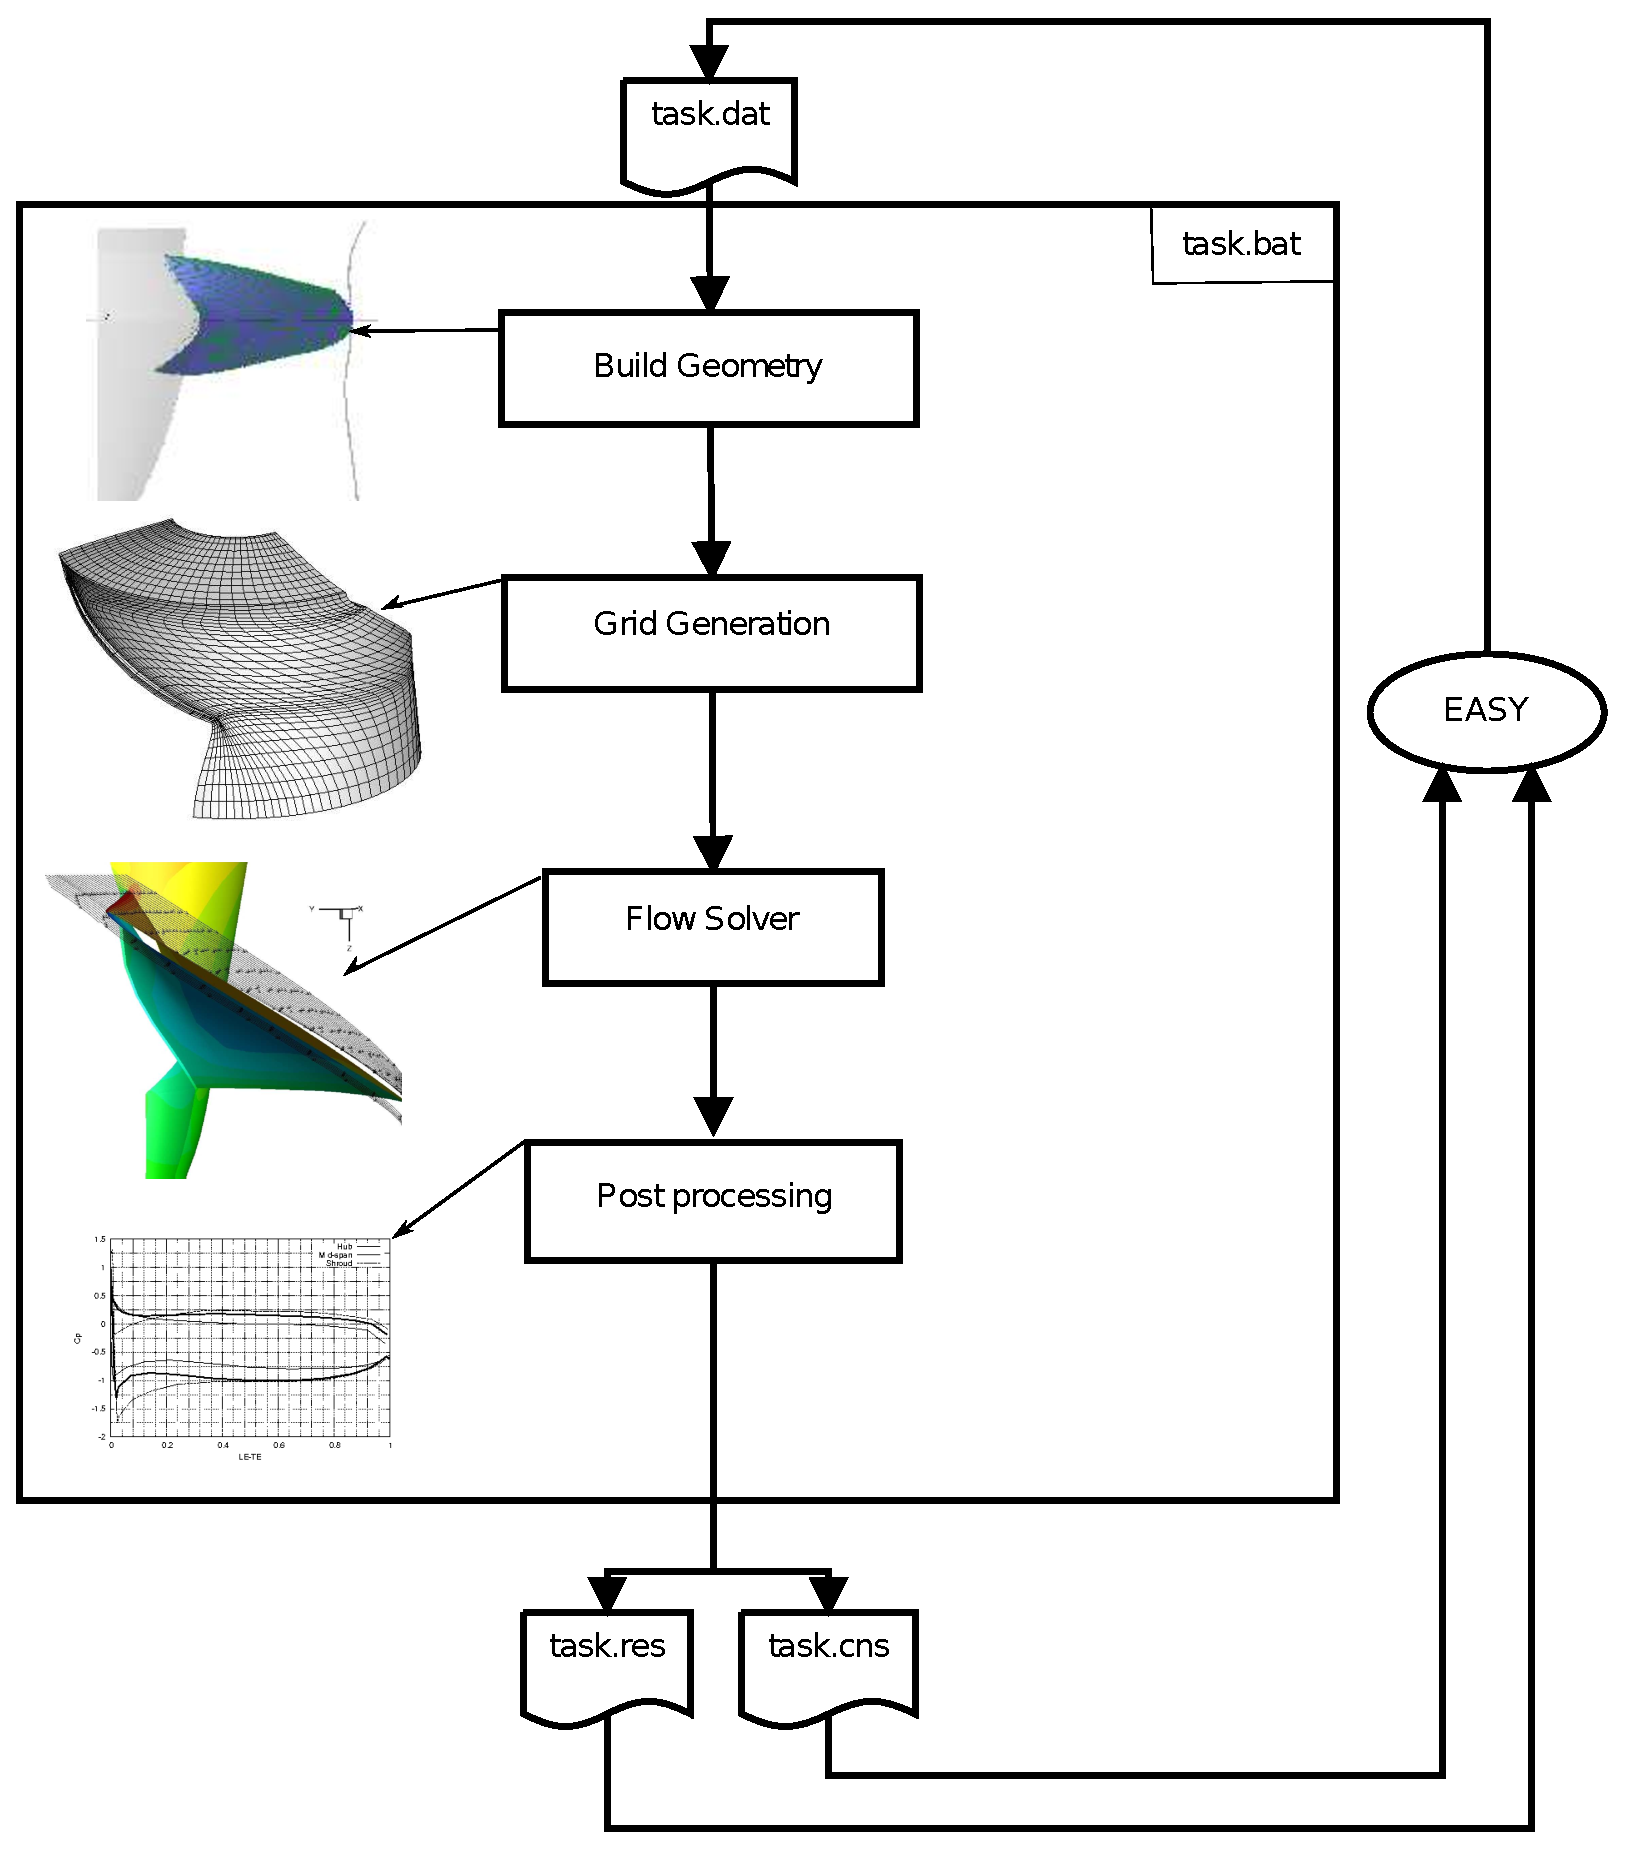
\includegraphics[width=135mm]{Optimizationloop.eps} 
\caption{According to the EASY nomenclature, the evaluation of each new candidate solution created during the evolution starts by reading the corresponding values of the design variables from the ``task.dat" file. A series of codes, being I/O compatible, are sequentially used to, finally, create the ``task.res" and ``task.cns" files which include the objective and constraint function values, respectively. The evaluation process is considered to be terminated once the ``task.res" and ``task.cns" files  become available to the search engine of EASY. The names of the executable files required for a single evaluation are listed in the script file "task.bat". }
\label{evaltool}
\end{figure}      


Post-processing is an indispensable part of the evaluation procedure. Post-processing tools are used to compute the metrics associated with the fitness of each candidate solution, as presented in section \ref{metrics}. 

Two problems are examined. The first problem is  dealing with the design-optimization of a Francis turbine runner to be installed in a pre-existing hydroelectric plant. This study is mainly used to study the gain from the use of the developed KBD method (Chapter \ref{KBDchapter}), as compared with the conventional EA, in an industrial environment where archived past designs, i.e. the outcomes of more or less similar projects, are, in fact, available.

The second problem is related to the design of a new type of hydraulic turbines, the so-called Hydromatrix$\circledR$. This case is used to demonstrate the gain from the implementation of the PCA-driven evolution operators (MAEA(PCA)), as compared with standard MAEA.     

      
\section{Evaluation Procedure}
\label{ParamEval}
\subsection{Parameterization for Turbine Blades}
\label{Paramt}
The  parameterization of a hydraulic turbine blade, of axial radial or mixed flow type, consists of two steps. The first step is the parameterization of its 3D mean-camber surface. The second step is concerned with the thickness of the blade which is defined by the airfoil shape and the thickness distribution across the blade, \cite{dipl_livia,dipl_simon}.

Starting point of the parameterization of the mean-camber surface is its meridional projection. The meridional projection of the mean-camber surface is confined by 4 curves, namely the hub and shroud generatrices, the leading and trailing edge curves (fig.\ \ref{param1}). All four curves are parameterized by a user-defined number of \Bezier\ control points.


%\begin{figure}[h!]
%\centering
%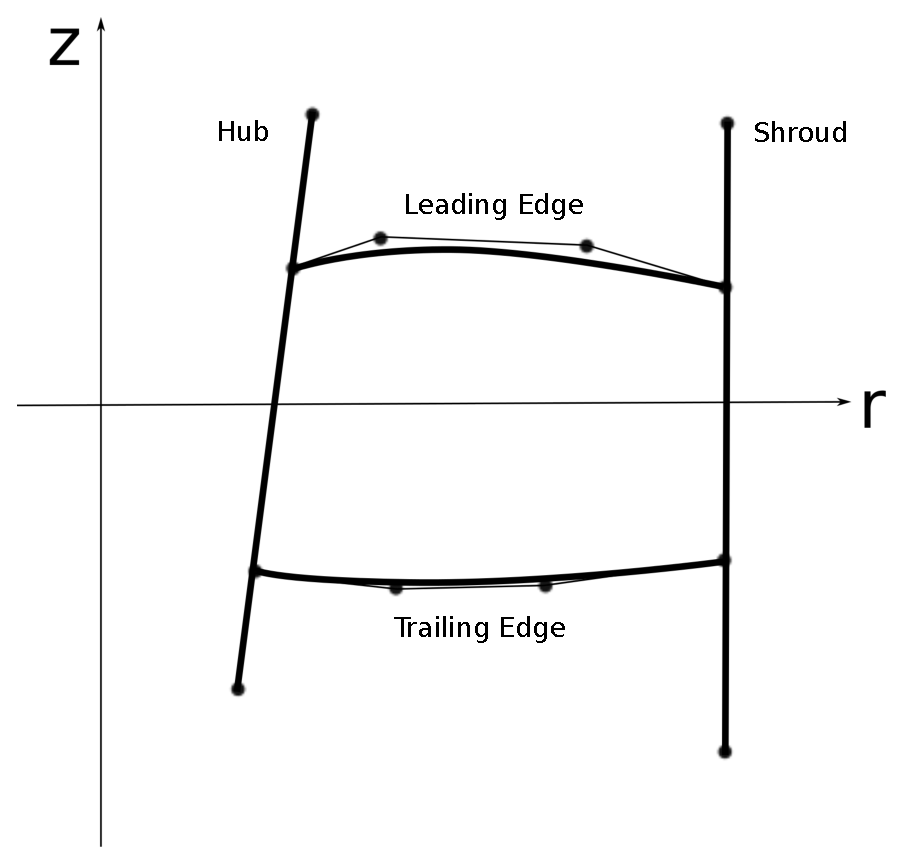
\includegraphics[width=100mm]{param1.eps} 
%\caption{Example of a meridional surface (here a Matrix blade) in cylindrical coordinates (r,z,f=0)}
%\label{param1}
%\end{figure}

Having defined the meridional projection of the mean-camber surface,  the generation of the 3D shape of the mean-camber surface follows. A set of 2D iso-span lines, distributed between the shroud and hub,  are generated (fig.\ \ref{param1}). The 3D shape of the aforementioned lines is  based on their meridional projection and a number of parameters, namely $\rho,\theta,\beta,\zeta$ and $\mu$, which are all defined below. These 3D lines are, then, used as the skeleton of the blade mean-camber surface (fig.\ \ref{param3}).

\begin{figure}[h!]
\begin{minipage}[b]{0.5\linewidth}
 \centering
 \resizebox*{6.5cm}{!}{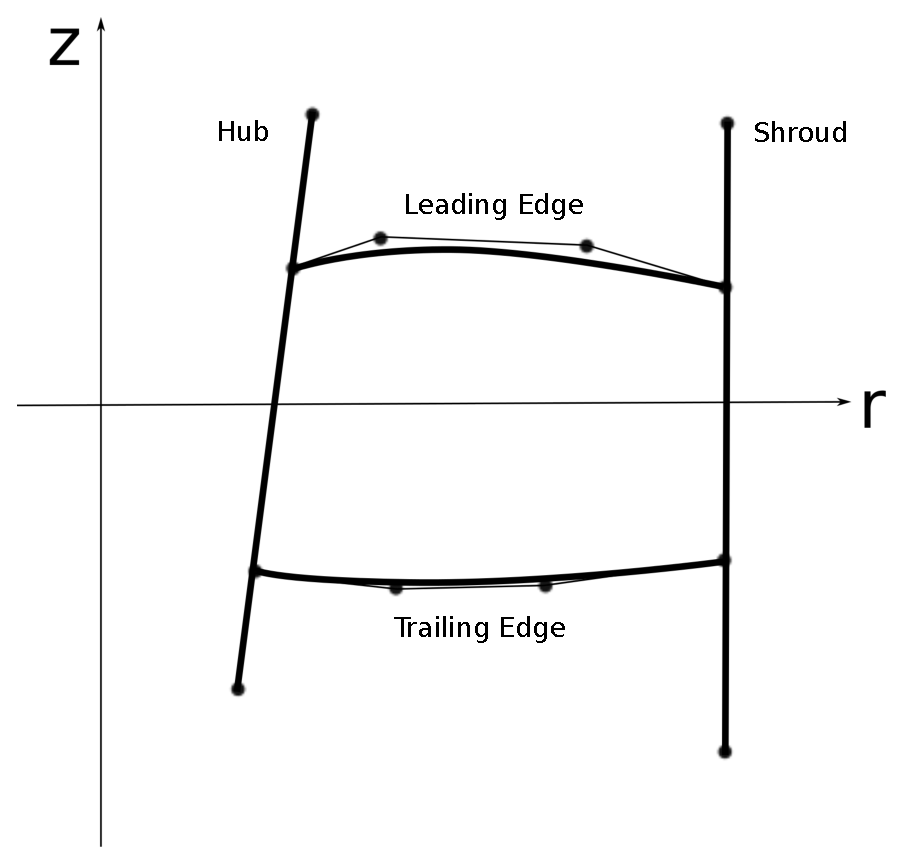
\includegraphics{param1.eps}}
\end{minipage}
\begin{minipage}[b]{0.5\linewidth}
 \centering
 \resizebox*{6.5cm}{!}{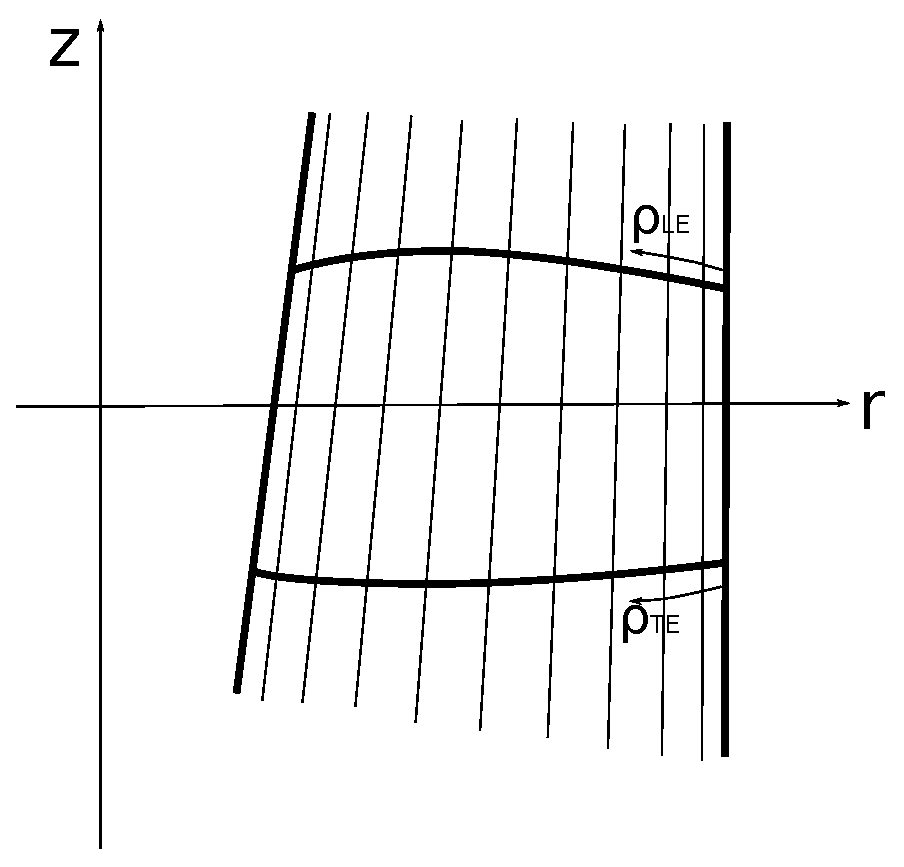
\includegraphics{param2.eps}}
\end{minipage}
\caption{Left: Meridional projection of the mean-camber surface of a HYDROMATRIX$\circledR$ blade. Right: The 2D iso-span lines distributed between shroud and hub. Definition of $\rho$ for the leading and trailing edge.}
\label{param1}
\end{figure}
 

%\begin{figure}[h!]
%\centering
%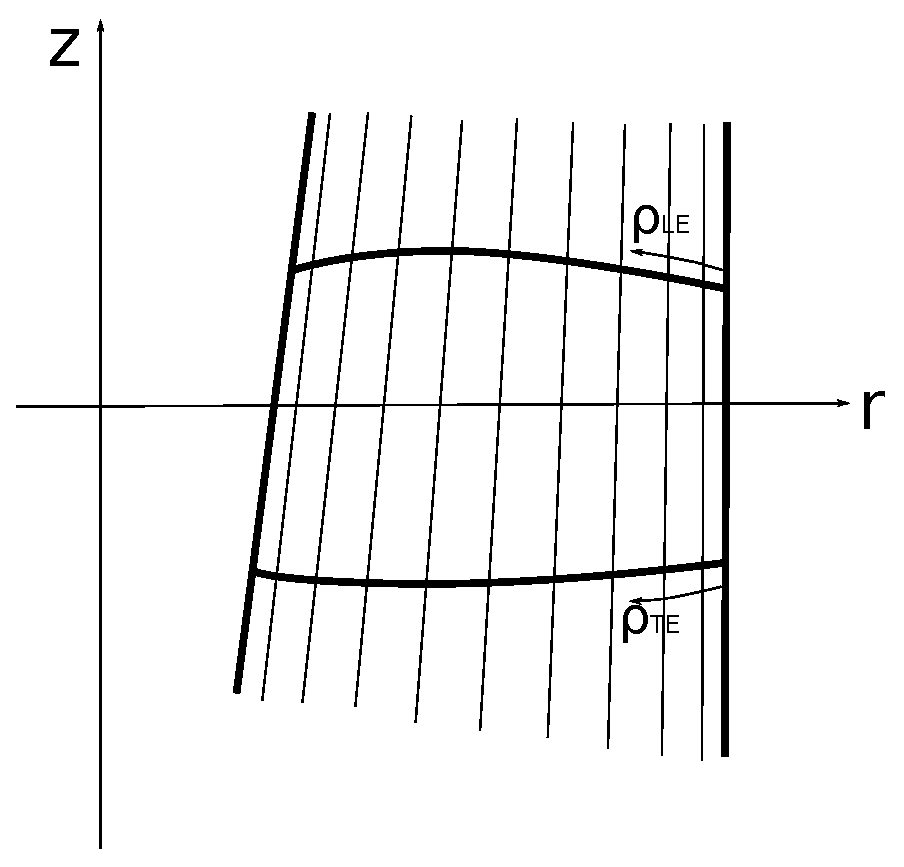
\includegraphics[width=100mm]{param2.eps} 
%\caption{Example of a 2-dimensional streamlines distribution between shroud and hub (here 11 streamlines). %Definition of $\rho$.}
%\label{param2}
%\end{figure}

The $\rho$ value is defined at each point along both the leading (LE) and trailing (TE) edges as the normalized meridional projection arc-length of the edge, with zero value at the shroud and unit value at the hub (fig.\ \ref{param1}). 

\begin{figure}[h!]
\centering
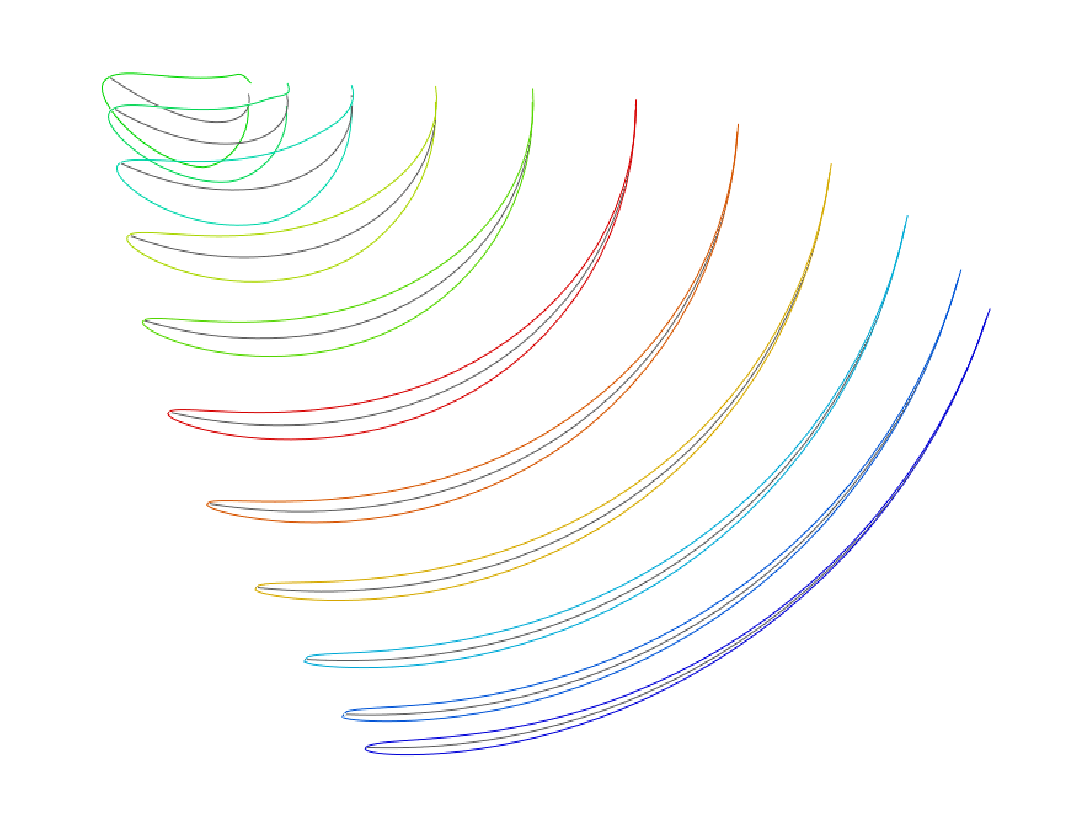
\includegraphics[width=120mm]{param3.eps} 
\caption{The 3D iso-span lines and their superimposed thickness profiles.}
\label{param3}
\end{figure}

The angular position of the LE and TE is controlled by the so-called wrap-around angle $\theta$. % is defined as the angle between the projected linear connection of a mean-surface-point and the z-axis onto the x-y-plane and the x-axis.
$\theta(\rho)$ distributions for the LE and TE together with the r and z values of their meridional projections define the final 3D shape of both edges. On the other hand, $\beta$ is defined as the angle between the local tangent to the mean-camber surface and the tangent to the z-centered circle through this point. Therefore, the $\beta(\rho)$ distributions define the mean-camber surface metal angles throughout the previously defined LE and TE. $\beta(\rho)$ and $\theta(\rho)$ distributions are parameterized as \Bezier\ curves of a user-defined degree (fig.\ \ref{param4}).  


\begin{figure}[h!]
\begin{minipage}[b]{1\linewidth}
 \centering
 \resizebox*{14cm}{!}{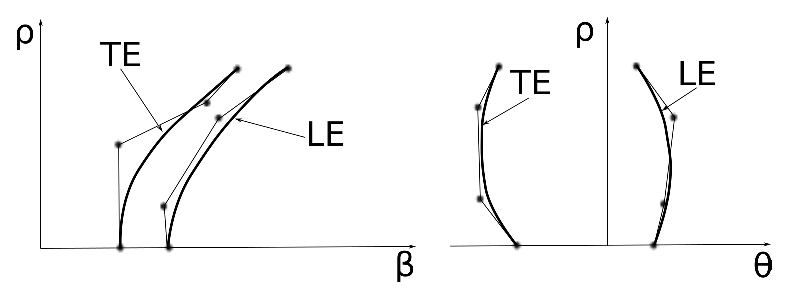
\includegraphics{param4_5.eps}}
\end{minipage}
%\begin{minipage}[b]{0.5\linewidth}
% \centering
% \resizebox*{6.5cm}{!}{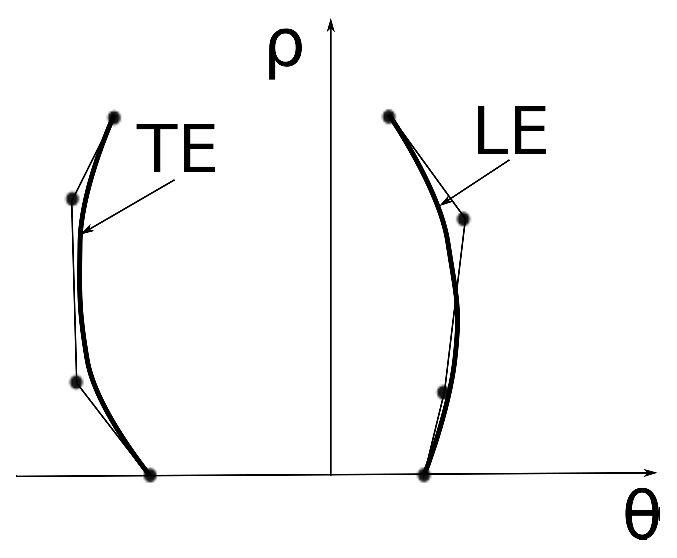
\includegraphics{param5.eps}}
%\end{minipage}
\caption{Left: $\beta(\rho)$ distribution. Right: $\theta(\rho)$ distribution.}
\label{param4}
\end{figure}

The final step in the parameterization of the mean-camber surface is to define its shape between the LE and TE for all the iso-span lines. This is achieved through the conformal mapping $\Phi$


\begin{equation} 
   \Phi:(r,z)\rightarrow \mu, ~~~~\mu=\int{\frac{1}{r}dl}
   \label{phi1} 
\end{equation}
where $l$ denotes the arc-length of the meridional projection of the iso-span line. This conformal mapping performs the transformation of the iso-span lines from the cylindrical  $(r,z,\theta)$ to the $(\mu,\theta)$ coordinate system. The iso-span lines (in the $(\mu,\theta)$ coordinate system) are defined by third-degree \Bezier\ curves. The first and last control points are fixed on the LE and TE points of each iso-span line and the two internal control points depend on $\zeta_{LE}, ~\zeta_{TE}, ~\beta_{LE}$ and $\beta_{TE}$ angles, respectively (fig.\ \ref{param7}).
  
Finally, the two $\zeta(\rho)$ distributions, for the LE ($\zeta_{LE}$) and TE ($\zeta_{TE}$), define the position of the two internal control points for all the iso-span lines ($0\leq\rho\leq1$). Therefore, the $\zeta$ distributions can be seen as the curvature control system of the aforementioned parameterization of the mean-camber surface scheme, since it defines how strongly the $\beta$ values at LE and TE affect the $\beta$ values in the interior of the mean-camber surface. Similar to $\theta(\rho)$ and $\beta(\rho)$, the $\zeta(\rho)$ distributions are also parameterized as \Bezier\ curves of a user-defined degree (fig.\ \ref{param7}). Then the  inverse conformal mapping $\Phi^{-1}$ is used to transform the iso-span lines from the $(\mu,\theta)$ coordinate system back to the cylindrical one. 

\begin{figure}[h!]
\begin{minipage}[b]{1\linewidth}
 \centering
 \resizebox*{14cm}{!}{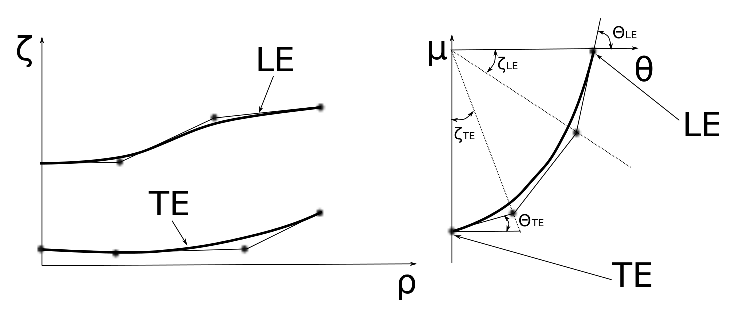
\includegraphics{param6_7.eps}}
\end{minipage}
%\begin{minipage}[b]{0.5\linewidth}
% \centering
% \resizebox*{7.5cm}{!}{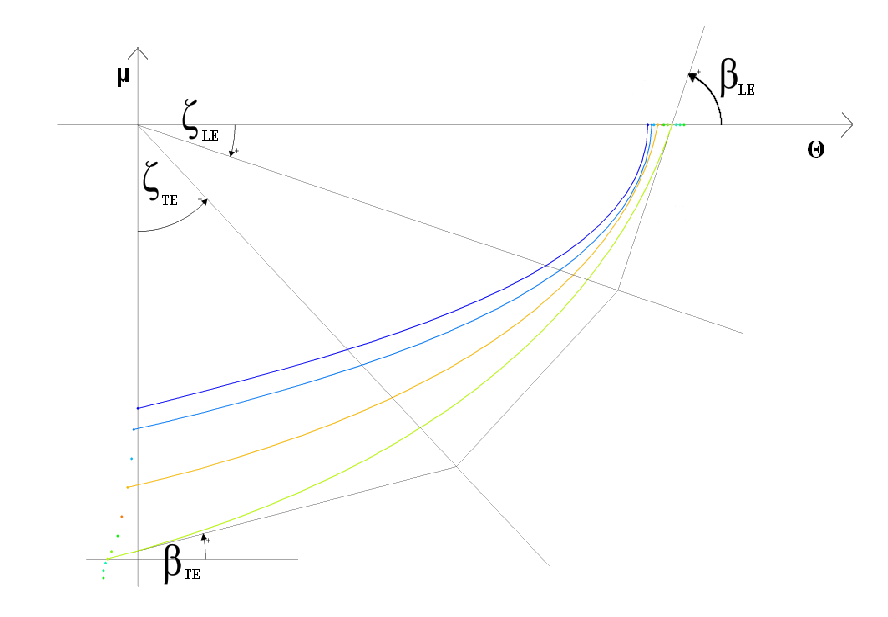
\includegraphics{param7.eps}}
%\end{minipage}
\caption{Left: $\zeta(\rho)$ distributions for $\zeta_{LE}$ and $\zeta_{TE}$. Right: Iso-span line, in the $(\mu,\theta)$ coordinate system, and its \Bezier\ control point polygon.}
\label{param7}
\end{figure}

The airfoil profiles are defined by a user-defined number of \Bezier\ points (fig.\ \ref{param8}) and the absolute thickness by two thickness (t($\rho$)) distributions (fig.\ \ref{param10}) (separately for the SS and PS). The airfoil profiles are scaled so that their maximum thickness be equal to the one specified by the t($\rho$) distribution. Finally, the scaled airfoil profiles are superimposed onto the mean-camber surface to create the final 3D blade (fig.\ \ref{param10}).  

\begin{figure}[h!]
\centering
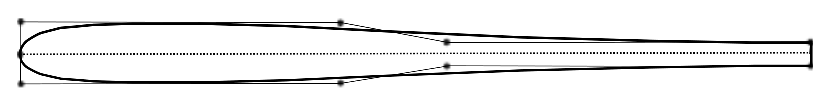
\includegraphics[width=150mm]{param8.eps} 
\caption{\Bezier\ control polygons for the PS and SS.}
\label{param8}
\end{figure}

%\begin{figure}[h!]
%\centering
%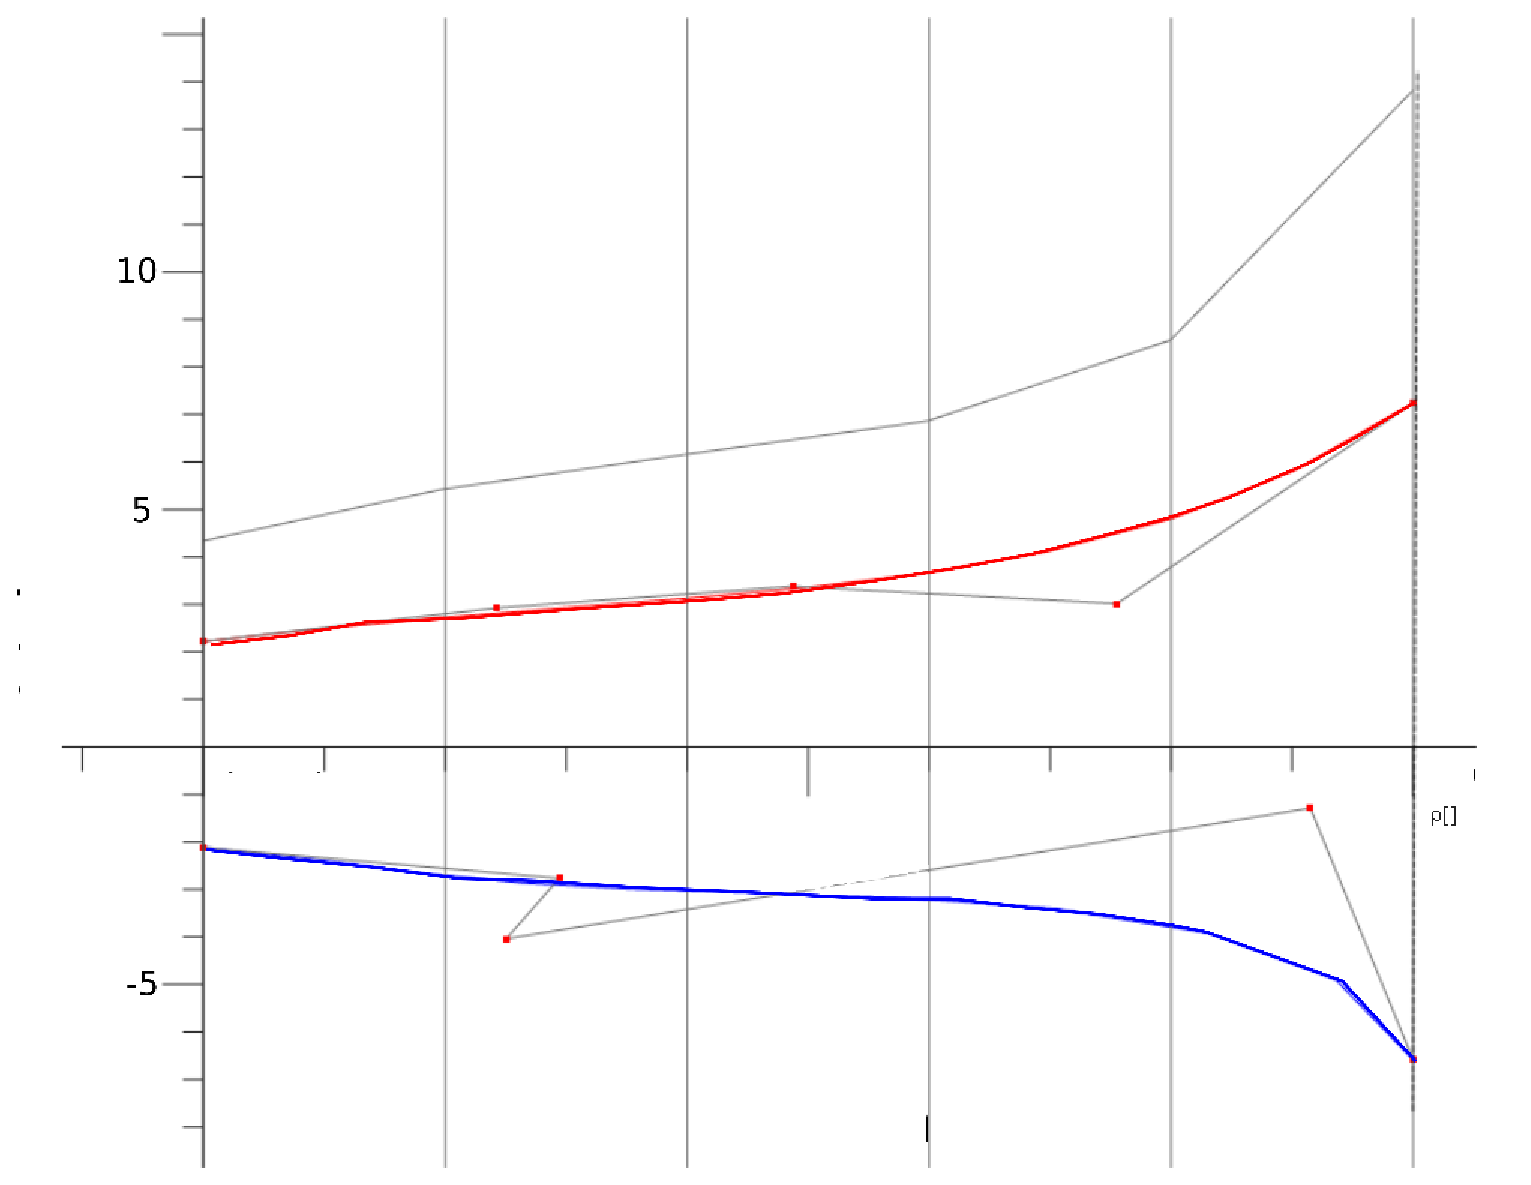
\includegraphics[width=60mm]{figure5.eps} 
%\caption{thickens-$\rho$ distribution.}
%\label{param9}
%\end{figure}


\begin{figure}[h!]
\begin{minipage}[b]{0.5\linewidth}
 \centering
 \resizebox*{6.5cm}{!}{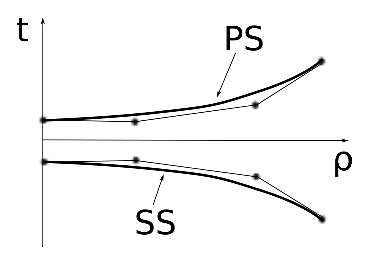
\includegraphics{param9.eps}}
\end{minipage}
\begin{minipage}[b]{0.5\linewidth}
 \centering
 \resizebox*{6.5cm}{!}{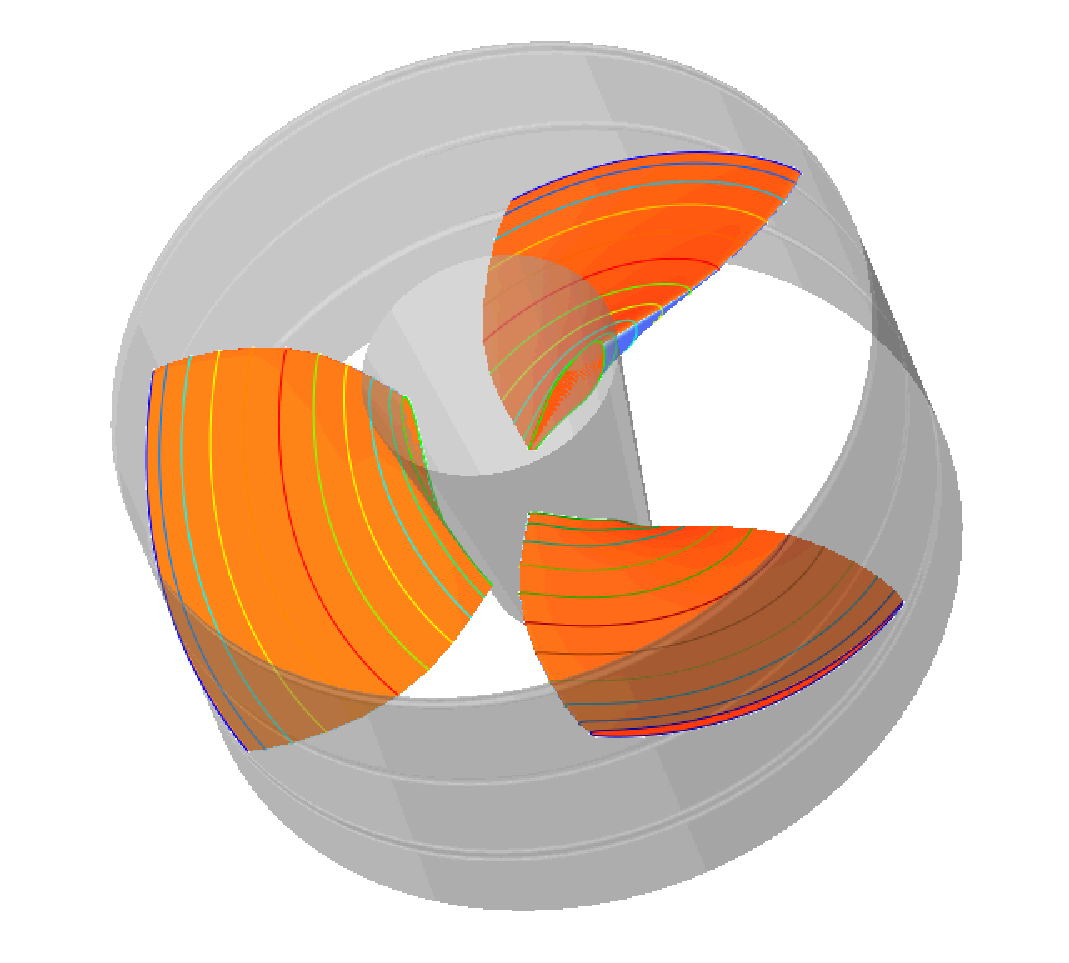
\includegraphics{param10.eps}}
\end{minipage}
\caption{Left: t($\rho$) distribution. Right: 3D geometry of a HYDROMATRIX$\circledR$ turbine with three blades.}
\label{param10}
\end{figure}

\FloatBarrier
\subsection{Space Discretization - Grid Generation}
\label{SpaceDisct}
A multi-block structured grid generator, tailor-made for hydraulic turbomachines, which has been developed by Andritz-ASROE is used. This is able to handle axial, radial and mixed flow machines. Structured grids, using blocks with fixed topology can, via stretching and twisting, create grids which fit the geometries under consideration. A multi-block topology (several interconnected structure grid blocks) gives maximum freedom to the user for generating grids around quite complex geometries (fig.\ \ref{grid1}). 


\begin{figure}[h!]
\centering
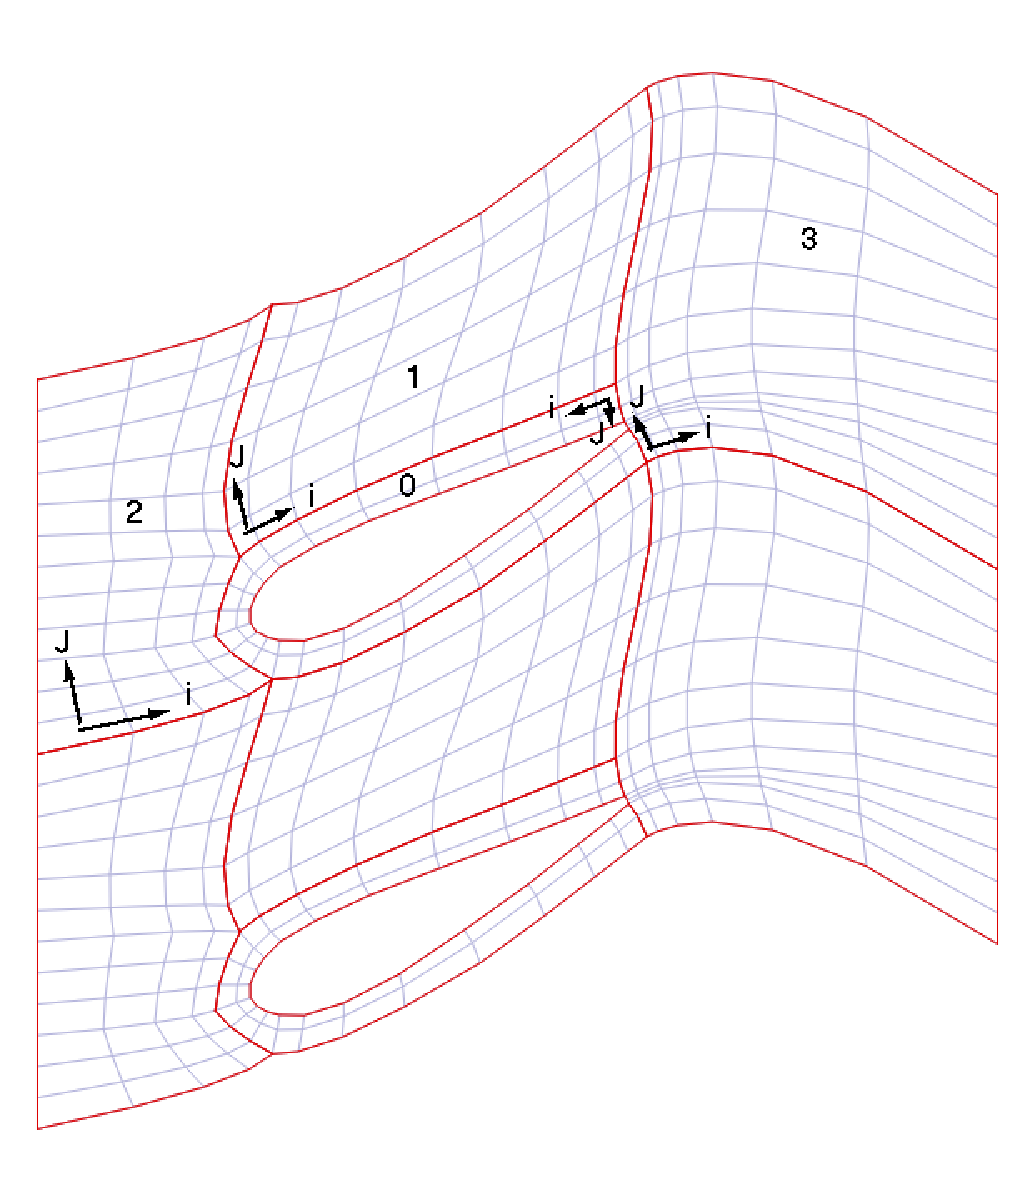
\includegraphics[width=100mm]{cGridSkBlockIndex.eps} 
\caption{The four-block topology of a hydraulic turbine. In the sake of simplicity, this is shown for the blade-to-blade grid at mid-span. Block 0 is of C-type and is used to discretize the area in the vicinity of the blade (airfoil). Blocks 1 to 3 are of H-type and are used to fill the space from pressure side to suction side, between LE and inlet and  blade TE and outlet, respectively; from \cite{PaulSite}.}
\label{grid1}
\end{figure}


In this thesis, with respect to the topological characteristics of hydraulic turbo-machines, such as the TE thickness and the extensions towards the inlet and outlet of the domain, a four-block topology is used,  fig.\ \ref{grid1}. Block 0 is of C-type and is used to mesh the area in the vicinity of the blade, capturing the TE thickness. Block 1 fills the space between two consecutive blades. Block 2 fills the space between the inlet and the blade LE. Finally, block 3 fills the space after blocks 0 and 1 up to the outlet. 

The user may control the grid via changing the shape of the block edges, defining number of nodes at each location % (fig.\ref{grid2}) 
 and the distribution of grid nodes at the domain boundaries.% (fig.\ref{grid3}).                      


%\begin{figure}[h!]
%\centering
%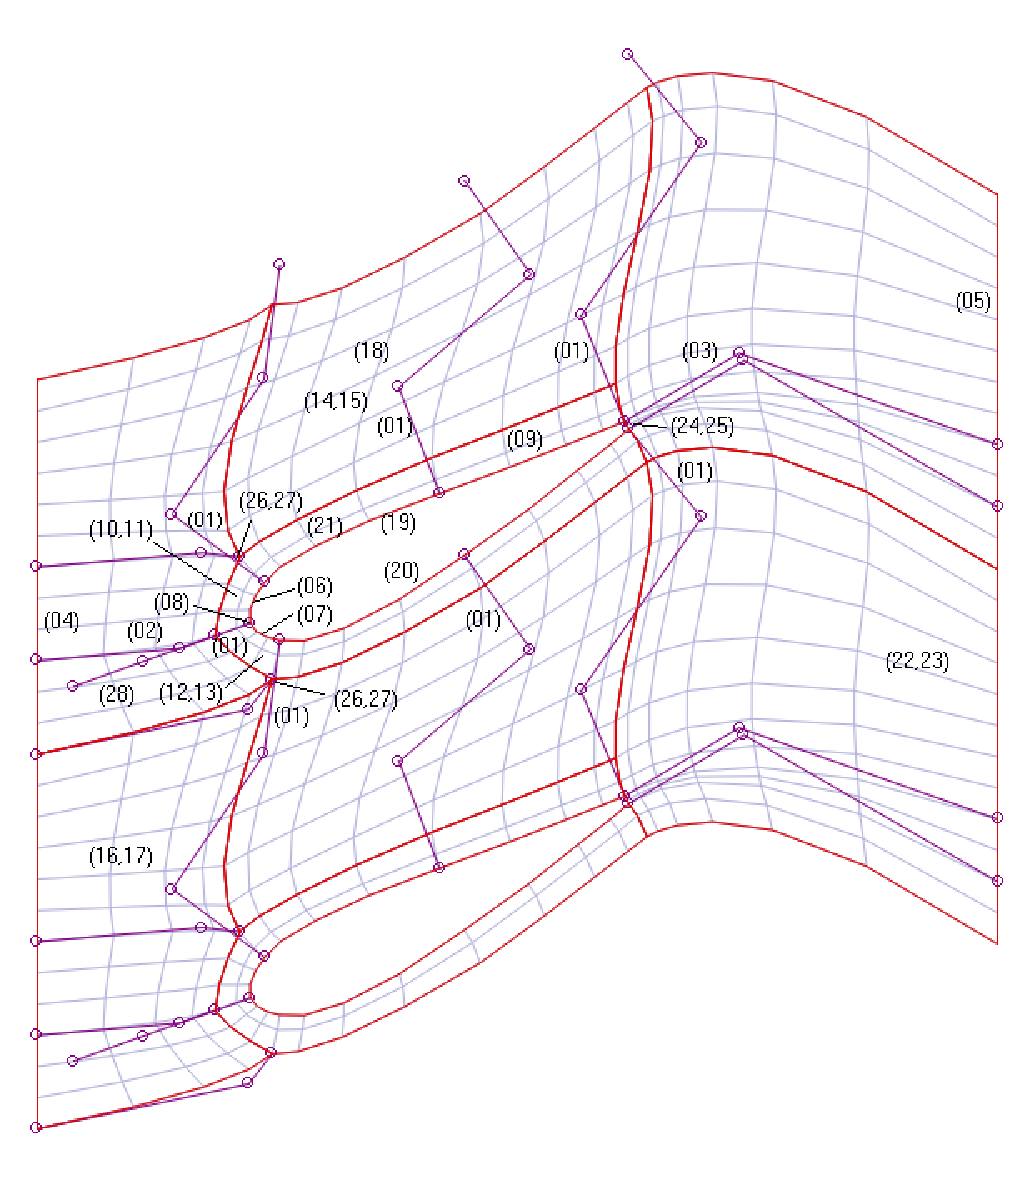
\includegraphics[width=100mm]{cGridSkParam.eps} 
%\caption{User-defined parameters controlling the shape of the block edges. These are a set of values constructed from a number of angles and distances that defined the control points of the figure. Numbers on these figure correspond to the number of the parameters and are depicted in the domains that they influence.}
%\label{grid2}
%\end{figure}

%\begin{figure}[h!]
%\centering
%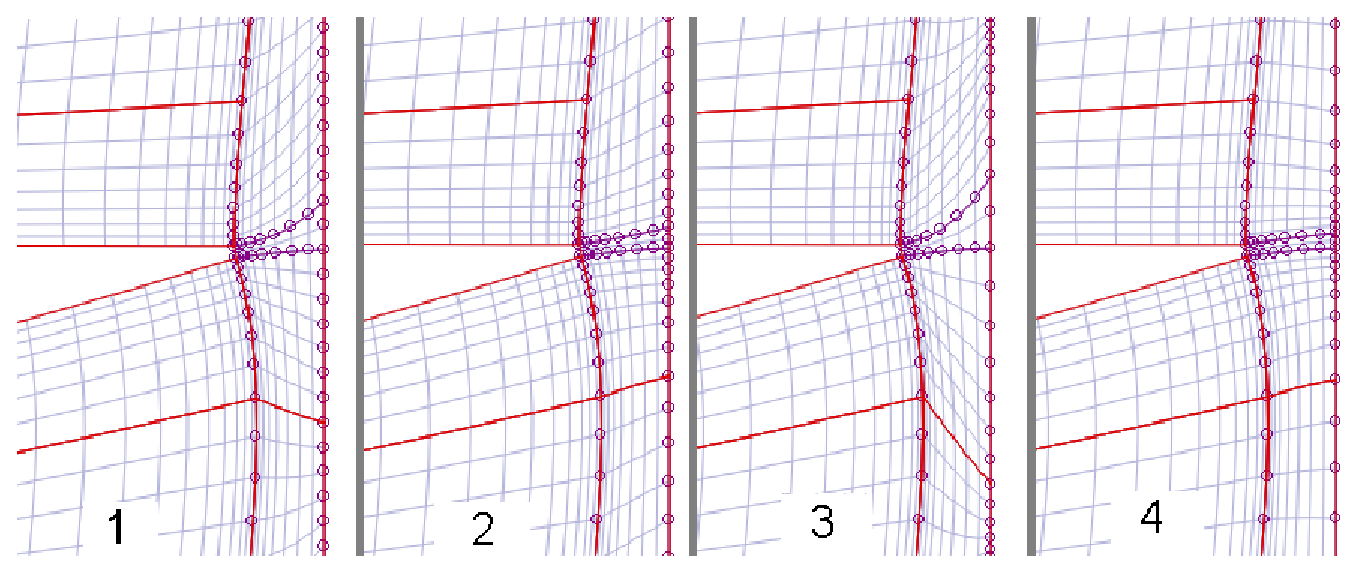
\includegraphics[width=120mm]{sketchDistrEast.eps} 
%\caption{Parameters controlling the distribution of grid-nodes along the domain-boundaries allow the user to place a greater number of points in regions of high gradients while reducing the number of grid nodes in regions with small gradients.}
%\label{grid3}
%\end{figure}

To construct the 3D grid, a user-defined number of pseudo 2D (laying on iso-span surfaces fig.\ \ref{grid4}) grids are computed using the grid parameterization as described above and are, then, combined to create the final 3D grid.

\begin{figure}[h!]
\centering
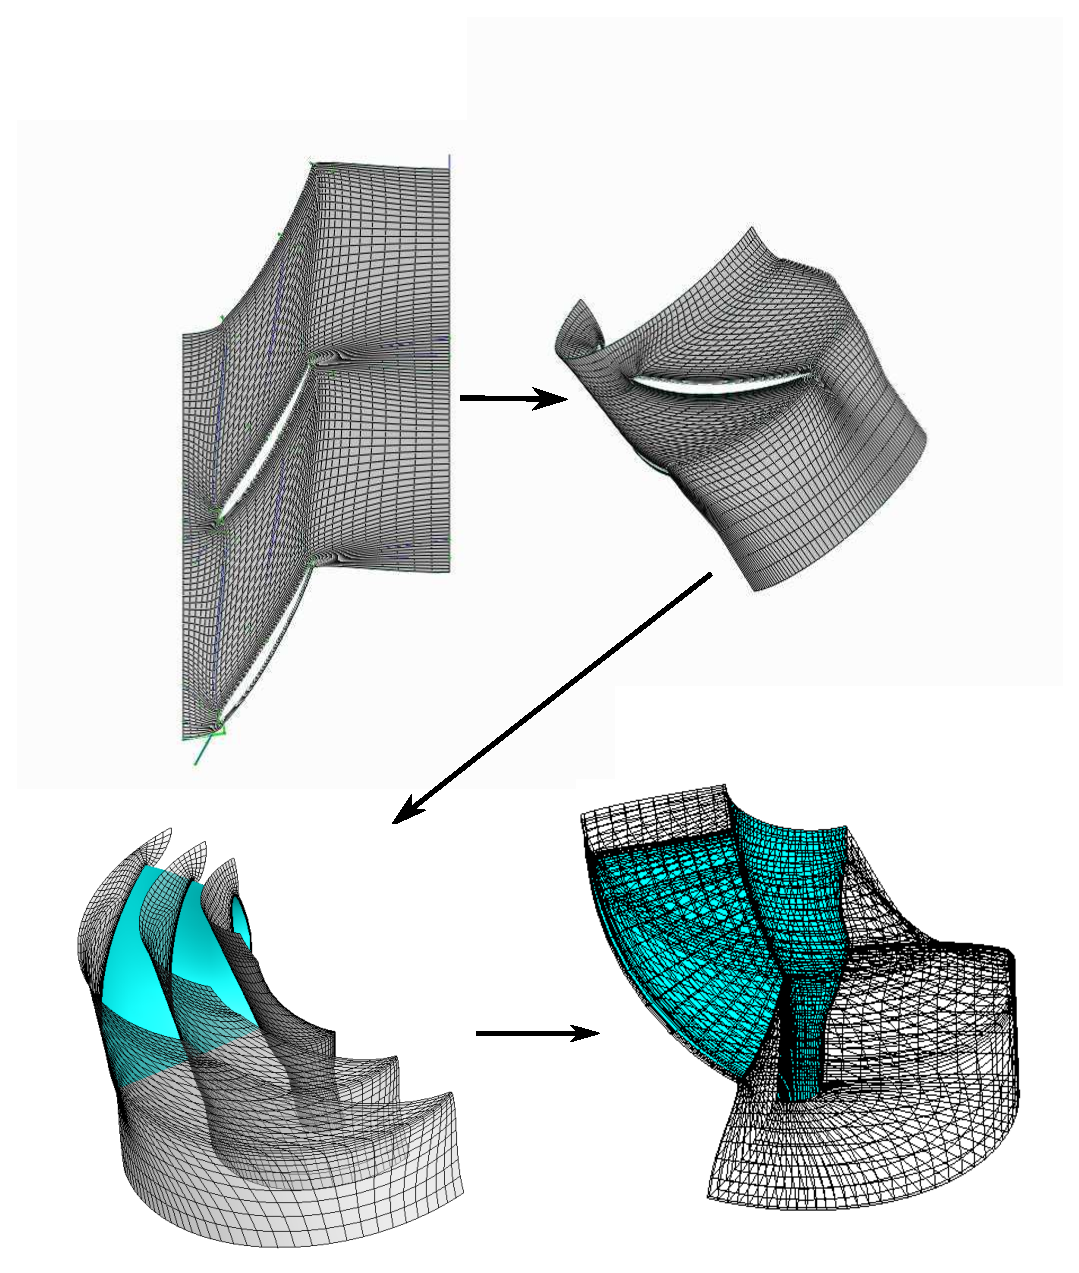
\includegraphics[width=140mm]{merid.eps} 
\caption{Iso-span surface grid, presented as a pseudo-2D grid. A user-defined number of the iso-span surface grids (from hub to shroud) is considered in order to generate the 3D grid. Top-Left: the pseudo-2D grid at the mid-span position. Top-Right: the same grid in the 3D space. Bottom-Left: Hub, mid-span and shroud grids. Bottom-Right: Final 3D grid.}
\label{grid4}
\end{figure}

It is important to mention that the described grid generation technique can accommodate a great variation of geometries without failing. This is of great importance for a grid generator to be used in an optimization loop. Thus, the risk of having ``good'' geometries classified as ``failed", due to the failure of the grid generation process, is minimized. 

In this thesis, both guide vane and runner blade channels are meshed using a grid generation tool with the previous features. 
%Typically, for speed sake, only one circumferential channel is computed (one guide vane and one runner channel with mixing plane interface).  

\FloatBarrier
\subsection{Flow Solver}
\label{FlowSolvert}
Water flow through the passage between the hydraulic turbine blades is simulated by a CFD code developed by Andritz-ASROE. The aforementioned code is a multiblock solver for the incompressible 3D Euler equations. The Euler equations are expanded by an artificial compressibility term, \cite{Chorin,Turkel87}. Their discretization is based on application of the 1D Roe approximate Riemann solver, \cite{Roe81}. The numerical solution is carried out by the ADI (Alternating Direction Implicit, \cite{Peaceman}) method on structured grids. Convergence is accelerated via a V-cycle multigrid scheme. The solver is developed for hydraulic turbomachines.

%using the 1D Roe approximate Riemann solver \cite{Roe81}
%is solving the Euler equations (eq. \ref{Euler1}) based on the artificial compressibility approach using the 1D Roe approximate Riemann solver \cite{Roe81}. For sake of wall time reduction this code employs a multi-grid solver. 

In differential form, the Euler equations with the artificial compressibility term are written as
\begin{equation} 
    \frac{\partial Q}{\partial t}=\nabla \cdot F
	\label{Euler1}
\end{equation}
where,
\begin{eqnarray}
		Q= \left( {\begin{array}{c}
 		p    \\
 		u_1  \\
 		u_2  \\
 		u_3  \\
 		\end{array} } \right)
 		, ~~ F_i= \left( {\begin{array}{c}
 		\beta ^2 u_i    \\
 		\beta ^2 u_1u_i + p\delta _1^i  \\
		\beta ^2 u_2u_i + p\delta _2^i  \\
 		\beta ^2 u_3u_i + p\delta _3^i  \\
 		\end{array} } \right)
\label{Euler3}
\end{eqnarray} 
where $\beta$ the artificial compressibility \cite{Chorin,Turkel87} and $\delta^i_j$ the Kronecker symbol.

Inlet and outlet boundary conditions are applied in an explicit way, on grouped faces, via the phantom cell technique. At the inlet, the total pressure distribution and the velocity angle or the velocity profiles are imposed. At the outlet, the static pressure or the total pressure, both based on the radial equilibrium equation, are imposed. 

Should the inlet velocity profile be imposed, the massflow is automatically determined and the hydraulic head results from the solution of the flow equations. On the the other hand, if the total pressure profile and velocity angle are defined at the inlet in combination with the total pressure and the radial equilibrium equation at the outlet, then the hydraulic head is fixed and the massflow results from the solution of the flow equations. Such a choice  plays a significant role regarding the control of the operating point, as it will be shown later on.        
%Using the above formulation each CFD calculation inside one runner channel takes only a few minutes. This fact and the observation that the influence of turbulence and viscosity are small enough allows, in combination with the proposed in this thesis techniques, the use of EAs as design tools in an industrial level i.e. with short (acceptable in a industrial environment) wall time. 

%Of coarse for the above statement to be true the appropriate objective functions, derived out of quality metrics that reflect the real quality of a runner and are not significantly influenced by turbulence and viscosity, have to be chosen. This type of metrics are presented, in detail, in section \ref{metrics} and will be used throughout this chapter. 
 
%In order to eliminate the obvious problem for incompressible flow (reduced state equation) an %artificial compressibility is introduced (cite R2 S5 ,maybe more). 

%The term $\frac{\partial \rho}{\partial t}$ is expanded by $\frac{\partial p}{\partial p}$, which results in 


%\begin{eqnarray}
%	\frac{\partial \rho}{\partial t} = \frac{\partial \rho}{\partial t}\frac{\partial p}{\partial p}
% = \frac{\partial p}{\partial t}\frac{1}{(\frac{\partial p}{\partial \rho})} 
% = \frac{\partial p}{\partial t}\frac{1}{\beta ^2}    
%\end{eqnarray}

%Thus the artificial compressibility $\beta$ is defined as;

%\begin{eqnarray}
%	\beta=\sqrt{\frac{\partial p}{\partial \rho}}
%\end{eqnarray}



\section{Hydraulic Turbine-Runner Quality Metrics}
\label{metrics}
The metrics used to quantify the quality of the candidate solutions are presented below. A metric may coincide with an objective function or a part of it or may even be used as a constraint.

In this thesis, metrics are associated with:
\begin{itemize}
\item{\textbf{\greek{σ:}}} The cavitation behaviour of the blade; cavitation is a common problem related to the operation of hydraulic machines subject to low pressure liquids, causing performance degradation and structural damages.
\item{\textbf{M$_1$:}} The circumferential and meridional velocity profiles at the exit position of the runner; the exit of the runner coincides with the inlet to the draft-tube and these profiles significantly affect the matching of the two components.
\item{\textbf{M$_2$}} The blade loading quality, since usually the equidistribution of loading is desired along the chordwise direction of the blade at any span-wise location.
\item{\textbf{M$_3$}} The pumping surface of the blade; in case of non-regulated turbines, neither the stator nor the rotor blade can be adjusted to perform optimally at every operating point. In such a case, during  part-load operation, a small part of the blade surface is operating as a pump, i.e. the PS has lower pressure than its SS; the corresponding surface is desired to be minimized.
\end{itemize}


\subsection{Cavitation Metric}
\label{cav.metric}
In hydraulic turbines, cavitation is the phenomenon of water vaporization (formation of cavities/bubbles) as the pressure tends to become lower than the vapour pressure. When the cavitation bubbles collapse in the vicinity of a solid surface, they may cause erosion, compromising thus both the structural integrity (removed material) and the hydraulic performance (altered shape) of the turbine \cite{thiruvengadam1974handbook,knapp1970cavitation,brennen1995cavitation}.  In addition, the collapse of cavitation bubbles generates noise, via the large momentary pressures that are generated when the internal of the bubble is highly compressed.

The conventional way to characterize how close the minimum liquid pressure is to the vapour pressure and, therefore, quantify the danger of cavitation to occur, is by means of the so-called cavitation number $\sigma$, defined as

\begin{eqnarray}
		\sigma=\frac{p_{\infty}-p_{v,T_{\infty}}}{0.5\rho_{L}U^2_{\infty}}
\label{Cavi}
\end{eqnarray}
where $U_{\infty}$, $p_{\infty}$ and $T_{\infty}$ stand for a reference velocity, pressure and temperature, respectively. $\rho_{L}$ is the liquid density and $p_{v,T_{\infty}}$  is the saturated vapour pressure. 

If $\sigma$ is sufficiently large, $p_{\infty}$ is large compared to $p_{v,T_{\infty}}$ or $U_{\infty}$ (eq.\ \ref{Cavi}), single-phase liquid flow will occur. However, if $\sigma$ drops below the $\sigma$ incipient value ($\sigma_i$), cavitation will occur. In the simplified case of a liquid which cannot withstand any tension and in which vapour bubbles appear instantaneously when the minimum pressure ($p_{min}$) reaches $p_{v}$,

\begin{eqnarray}
		\sigma_i=\frac{p_{\infty}-p_{min}}{0.5\rho_{L}U^2_{\infty}}
\label{Cavi2}
\end{eqnarray}
The incipient cavitation number could be ascertained from observations, measurements or simulations of the single-phase flow. For $\sigma > \sigma_i$, the pressure along the entire flow field is greater than $p_v$ thus no cavitation occurs. On the other hand, if $\sigma \leq \sigma_i$, it exists at least one point in the flow field with pressure lower than $p_v$ where cavitation occurs. 


For hydraulic turbines, the tendency of the flow to cavitate is characterized by the so-called Thoma's cavitation coefficient $\sigma$, \cite{brennen1995cavitation}  
\begin{eqnarray}
		\sigma=\frac{p_{t,exit}-p_{v}}{\rho_{L}gH}
\label{Cavi3}
\end{eqnarray}
where $p_{t,exit}$ is the total pressure at the exit of the turbine, $p_v$ the vapour pressure for the liquid and $H$ the hydraulic turbine head. The denominator is the total pressure difference between the turbines inlet and outlet.   

Making the same assumptions as in eq. \ref{Cavi2}, the $\sigma_i$ for the Thoma's cavitation coefficient  is 

\begin{eqnarray}
		\sigma_i=\frac{p_{t,exit}-p_{min}}{\rho_{L}gH}
\label{Cavi4}
\end{eqnarray}
Let $C_p$ be the pressure coefficient 
\begin{eqnarray}
		C_p=\frac{p-p_{t,exit}}{\rho_{L}gH}
\label{Cpdef}
\end{eqnarray}
The $\sigma_i$ quantity for the Thoma's cavitation coefficient is 
\begin{eqnarray}
		\sigma_i=-C_{pmin}
\label{Cavi6}
\end{eqnarray}
where $C_{pmin}$ is the $C_p$ value at the location where the minimum pressure ($p_{min}$) appears.

The cavitation behaviour of a hydraulic turbine can be observed through the $C_p$ distribution, plotted over the hydraulic turbine surfaces.  In fig.\ \ref{design-cav-cp}, the $C_p$ distribution of a turbine runner blade at mid-span is shown. There are , in fact, three possibilities: (a) $\sigma\!>\!-C_{pmin}$, thus $p_v\!<\!p_{min}$ and therefore cavitation doesn't occur; (b)  $\sigma\!=\!-C_{pmin}$, in which case if the assumptions of eq. \ref{Cavi2} and \ref{Cavi4} are true, the liquid cannot withstand any tension and vapour bubbles appear instantaneously when minimum pressure ($p_{min}$) reaches $p_{v}$, so cavitation occurs at the point of minimum pressure; (c) $\sigma\!<\!-C_{pmin}$, in which case $p\!<\!p_v$ over  part of the blade. Therefore, this region is considered as cavitated.     

\begin{figure}[h!]
\begin{minipage}[b]{1\linewidth}
 \centering
 \resizebox*{10cm}{!}{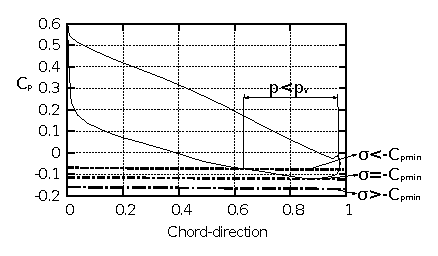
\includegraphics{CP2.eps}}
\end{minipage}
\caption{Pressure coefficient distribution at the blade mid-span.}
\label{design-cav-cp}
\end{figure}

In this thesis, in order to reduce the effects of assumptions related to eq.\ \ref{Cavi2} and eq. \ref{Cavi4}, the $\sigma$-histogram method \cite{Schmidl} is used. In the $\sigma$-histogram method, during the calculation of $\sigma_i$, the minimum pressure $p_{min}$ is replaced with the  so-called histogram pressure $p_{Hist}$ (eq.\ \ref{Cavi7}). $p_{Hist}$ is extracted from the blade pressure distribution, after require that a user-defined surface percentage (A) must have pressure values below $p_{Hist}$, (fig.\ \ref{design-cav-histo})  

\begin{eqnarray}
		\sigma_i^{Hist}=\frac{p_{tot,exit}-p_{Hist}}{\rho_{L}gH}
\label{Cavi7}
\end{eqnarray}
%where

%\begin{eqnarray}
%		A(p<p_{Hist})=A\%A_{Blade}
%\label{Cavi7}
%\end{eqnarray}

\begin{figure}[h!]
\begin{minipage}[b]{1\linewidth}
 \centering
 \resizebox*{10cm}{!}{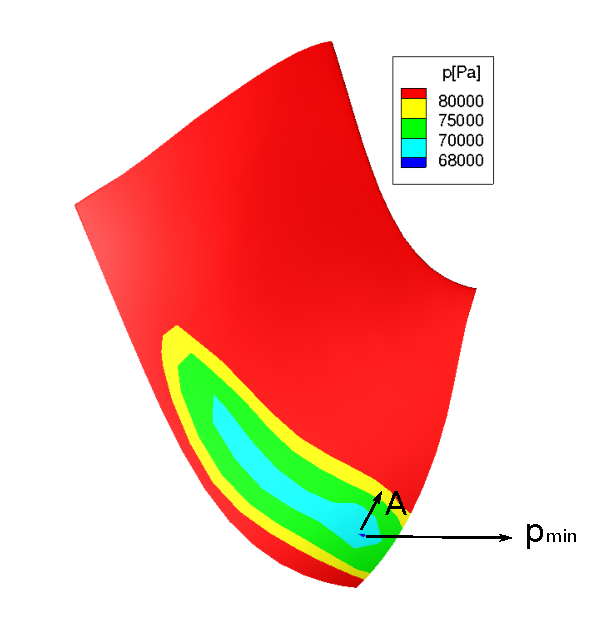
\includegraphics{histo.eps}}
\end{minipage}
\caption{$p_{Hist}$ computed with three different A values together with $p_{min}$ on the SS of a Francis hydraulic turbine. Increasing A results in increased $p_{Hist}$ and, therefore, reduced $\sigma_i^{Hist}$. The values of A used to plot this figure were artificially set quite different than the ones used in the optimization, in order to present visible iso-areas.}
\label{design-cav-histo}
\end{figure}

%\begin{figure}[h!]
%\begin{minipage}[b]{0.5\linewidth}
% \centering
% \resizebox*{7.5cm}{!}{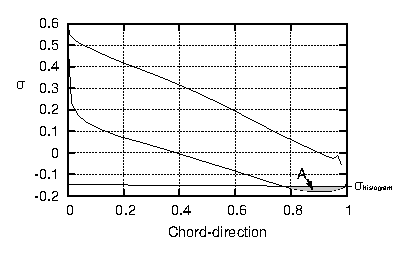
\includegraphics{sigma.eps}}
%\end{minipage}
%\begin{minipage}[b]{0.5\linewidth}
% \centering
% \resizebox*{6.0cm}{!}{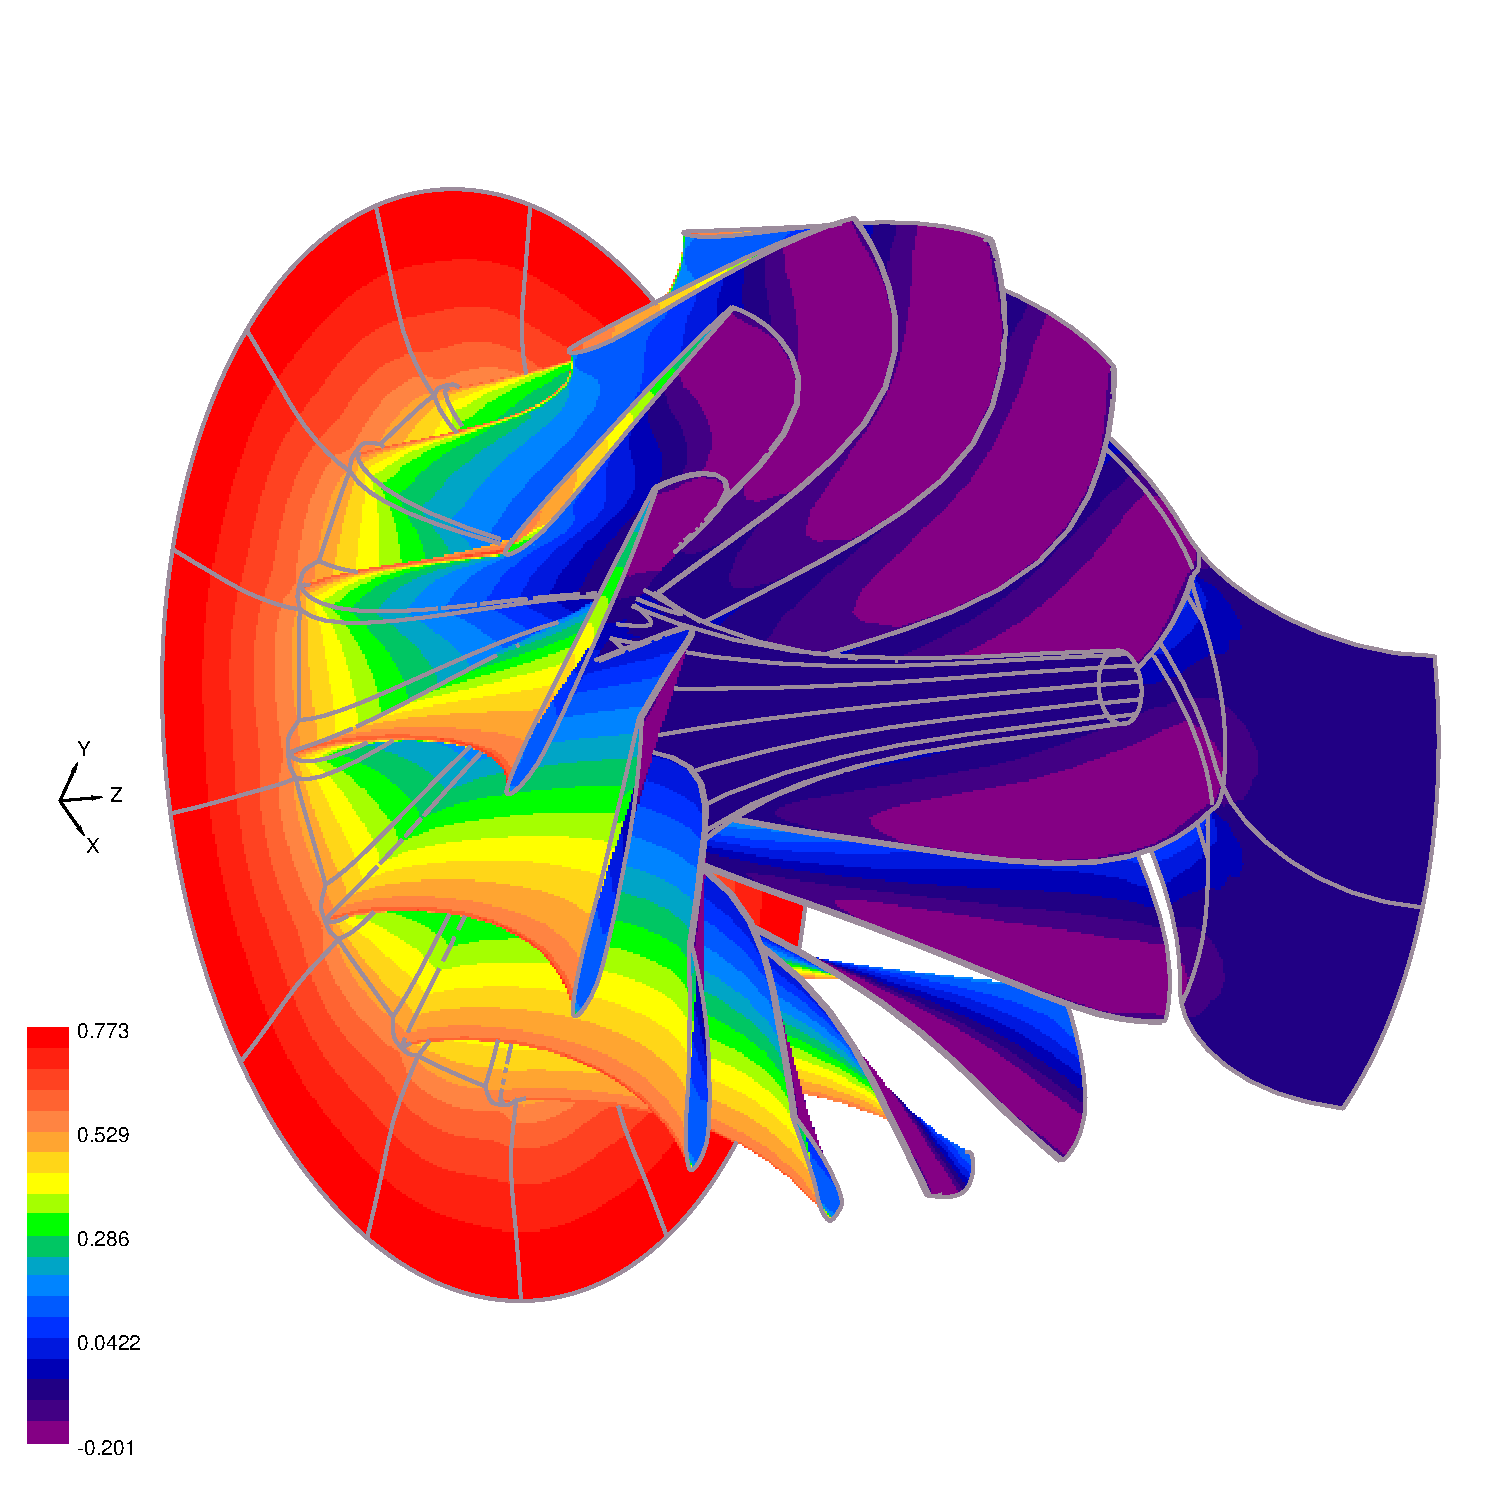
\includegraphics{Cavitation.eps}}
%\end{minipage}
%\caption{Left; $\sigma_{histogram}$ is equal to the $\sigma$ value for which a specific percentage of the blades surface "A" has lower pressure values than $p_{Hist}$, here A is set equal to $0.2\%$ of the blades surface, A is the blade surface that corresponds to the gray area here; Francis runner $\sigma$ contour plot. }
%\label{design-cav}
%\end{figure}


\subsection{Outlet Velocity Profiles}
Coupling the turbine runner with a pre-existing draft-tube is controlled via the outlet velocity profile metrics. This requires the definition of a target distribution and, thus, the corresponding metric stands for the deviation of the acquired distribution from the target one (fig.\ \ref{design-obj2}). To perform optimally, a given draft-tube must have specific mass-flow ($C_m=\frac{c_m}{\sqrt{2gH}}$) and  swirl ($C_u=\frac{c_u}{\sqrt{2gH}}$) span-wise distributions where, $c_m$ and $c_u$ are the meridional and circumferential components of the flow velocity, respectively.

%\begin{eqnarray}
%		C_m=\frac{c_m}{\sqrt{2gH}}
%\label{Cavi4}
%\end{eqnarray}
%and 
%\begin{eqnarray}
%		C_u=\frac{c_u}{\sqrt{2gH}}
%\label{Cavi4}
%\end{eqnarray}
%where $c_m$ and $c_u$ are the meridional and circumferential components of the flow velocity respectively.

Therefore, the  ``outlet velocity quality" metric is defined as the deviation of the computed distributions from the corresponding targets. 

\begin{figure}[h!]
\begin{minipage}[b]{1\linewidth}
 \centering
 \resizebox*{10.0cm}{!}{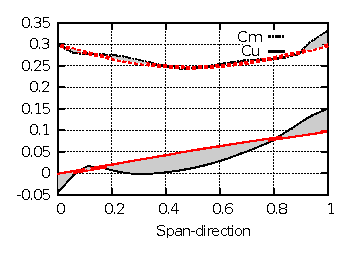
\includegraphics{OUTLET.eps}}
\end{minipage}
\caption{Outlet velocity distributions (thin lines) and the draft-tube specific target distributions (thick lines). $C_m$ is shown with the dashed lines and $C_u$ with the solid ones. The ``outlet quality" metric stands for the deviation between the computed distributions and the targets and is marked in grey.}
\label{design-obj2}
\end{figure}

%Even though allowing swirl at the runners outlet, as it is shown in figure \ref{design-obj2}, reduces its efficiency as an isolated part, it is needed to ensure the absence of flow detachment in the draft tube witch if happened would result in a dramatic drop in efficiency of the turbine as a hole.  



\subsection{Blade Loading Quality Metric}
Loading quality refers to the way load (eq. \ref{load}) is distributed along the runner blade surface. Constant load along the blade, in the chordwise direction, is desirable (fig.\ \ref{design-obj}) and is linked both to the hydraulic quality and the good structural behaviour. Load, at each blade position, is defined as the integral of pressure coefficient difference $(C_p^{PS}-C_p^{SS})$ over the blade surface 
%Chrodwise distribution of load for a given profile can be calculated via splitting the chord in $n$ equal segments of length $d_x$ then the load for every position of the chord can be calculated as; (fig.\ref{design-obj})     

\begin{align} 
   Load(x)=\int (C_p^{PS}(x)-C_p^{SS}(x)) dx 
\label{load}
\end{align}

%where,
%\begin{eqnarray}
%		C_p=\frac{P_{tot,exit}-P}{\rho_{L}gH}
%\label{Cpdef}
%\end{eqnarray}
%The $C_p$ definition used herein is equivalent with the $\sigma$ definition, see above, and will be used both to track Load quality and cavitation danger.  
  

\begin{figure}[h!]
\begin{minipage}[b]{0.5\linewidth}
 \centering
 \resizebox*{7.0cm}{!}{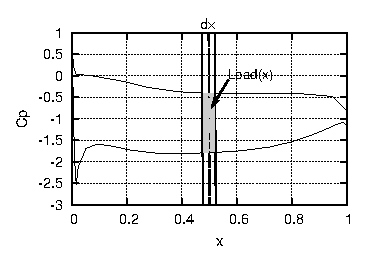
\includegraphics{CP.eps}}
\end{minipage}
\begin{minipage}[b]{0.5\linewidth}
 \centering
 \resizebox*{7.0cm}{!}{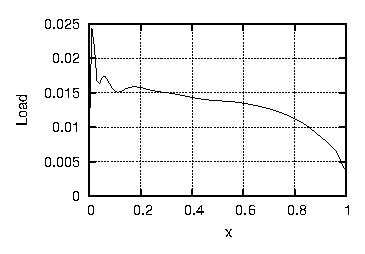
\includegraphics{Load.eps}}
\end{minipage}
\caption{Left: Load definition. Right: Chord-wise load distributions of the profile presented on the left, as defined before.}
\label{design-obj}
\end{figure}

Since constant load along the blade, in the chordwise direction, is desirable, optimization should aim at the minimization of the standard deviation of the load along the blade surface. 


\subsection{Pumping Surface Metric}
In case of non-regulated hydraulic turbines, such as the Hydromatrix$\circledR$ (section \ref{Matrix-case}), an extra quality metric which is associated with their operation at part-load, must be introduced.      

In non-regulated machines, neither the stator nor the rotor blades can be rotated so to adjust incoming/outgoing flow directions. During part-load operation, negative incidence angles appear (fig.\ \ref{design-pumpS}), creating thus a region where the SS has higher pressures than the PS. This part of the blade is operating as a pump and, in a well performing turbine, must be minimized. 

\begin{figure}[h!]
\begin{minipage}[b]{1\linewidth}
 \centering
 \resizebox*{10.0cm}{!}{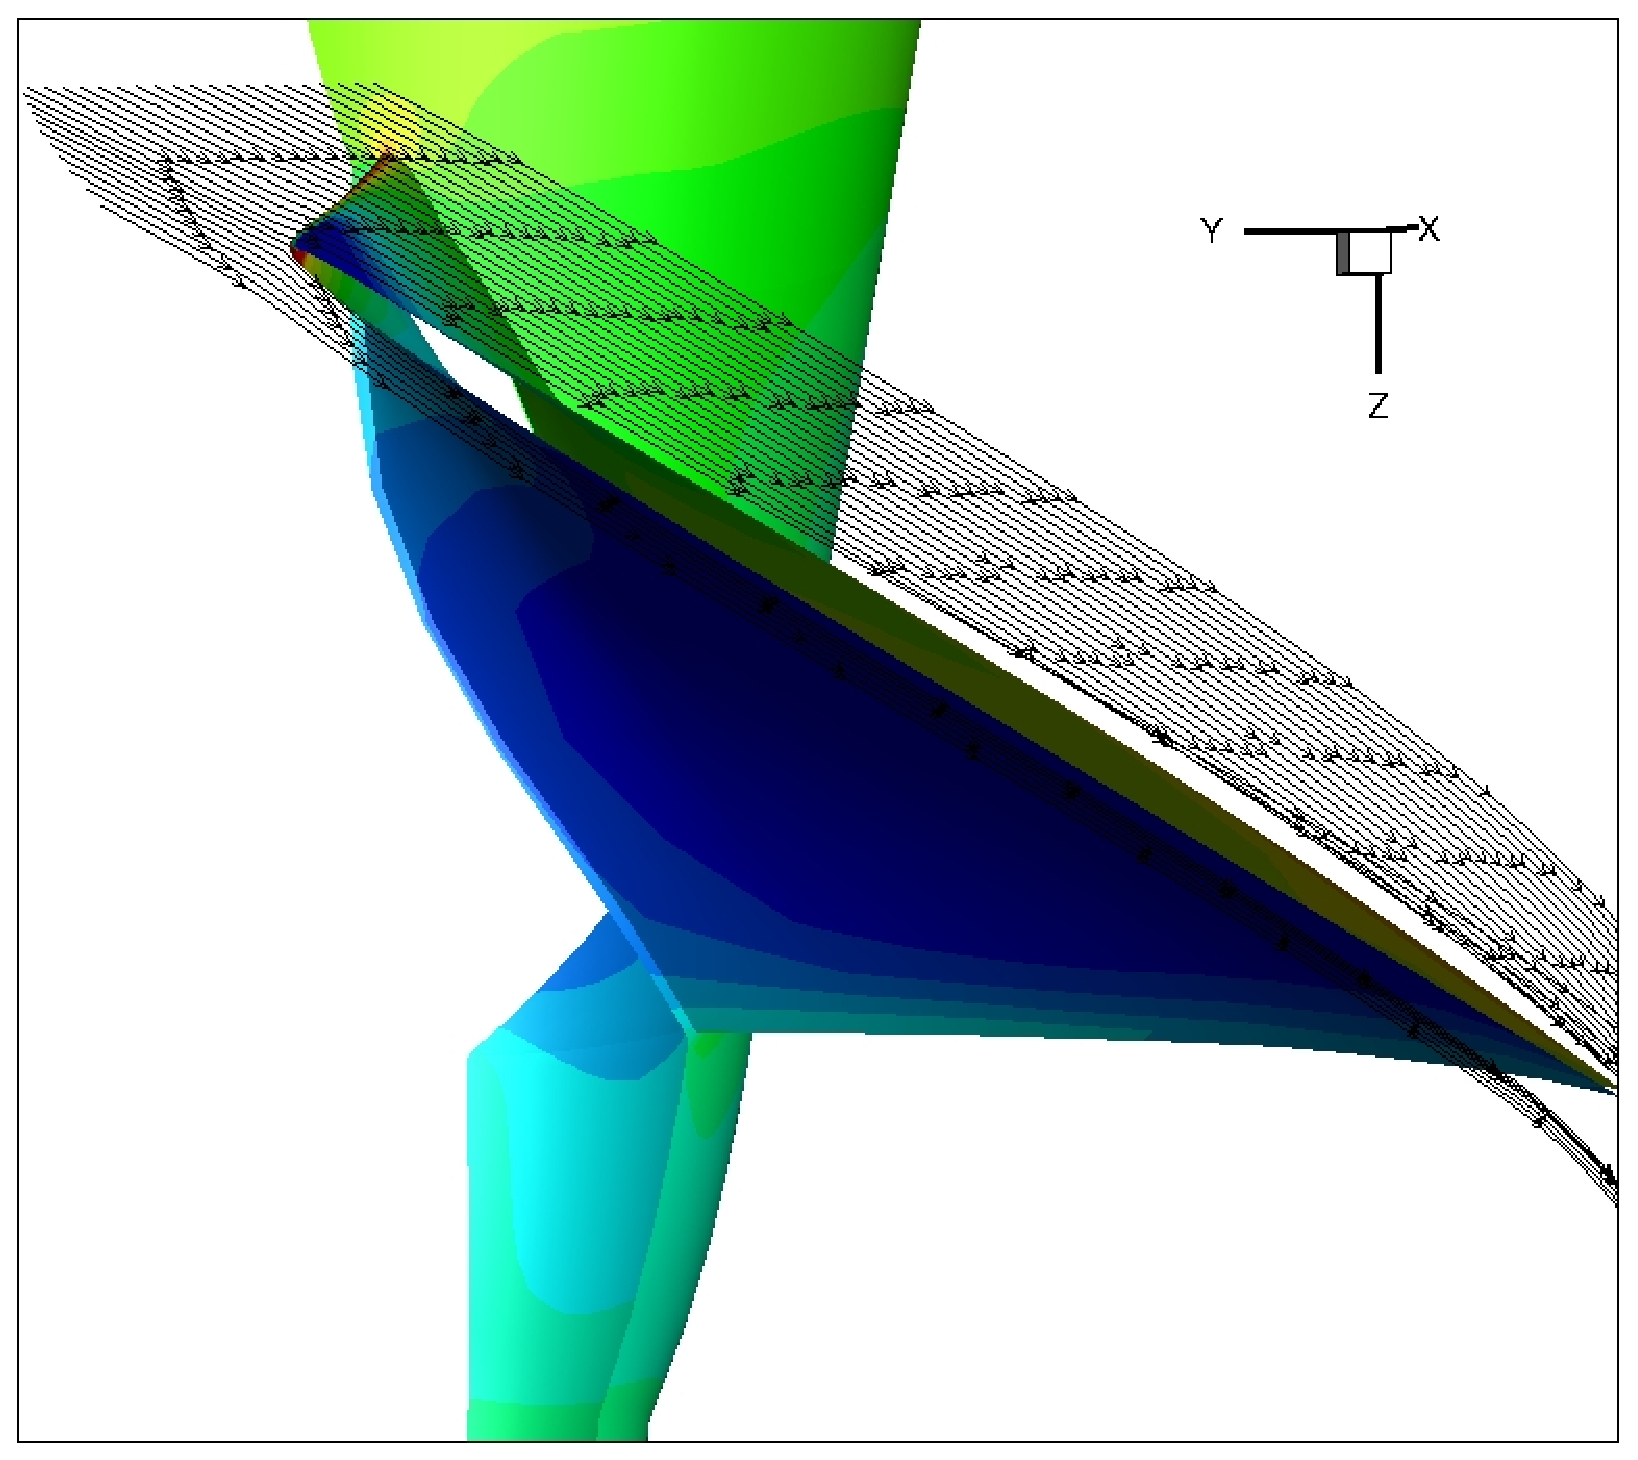
\includegraphics{PartLoad.eps}}
\end{minipage}
\caption{Pressure contour, along with streamlines near the shroud region, at part-load operation of a non-regulated hydraulic turbine. Water flow near the shroud region has negative incidence angle and, therefore the aforementioned pumping surface is formed. This surface needs to be minimized. The blade PS is the one on top.}
\label{design-pumpS}
\end{figure}

In fig.\ \ref{design-pumpS}, one may observe the flow streamlines at the near shroud region and how they meet the blade SS. This causes both a high-pressure region at the SS, due to the stagnation of the flow in there this meets the blade,  and a low pressure region on the PS due to high flow speeds.        

\begin{figure}[h!]
\begin{minipage}[b]{1\linewidth}
 \centering
 \resizebox*{14.0cm}{!}{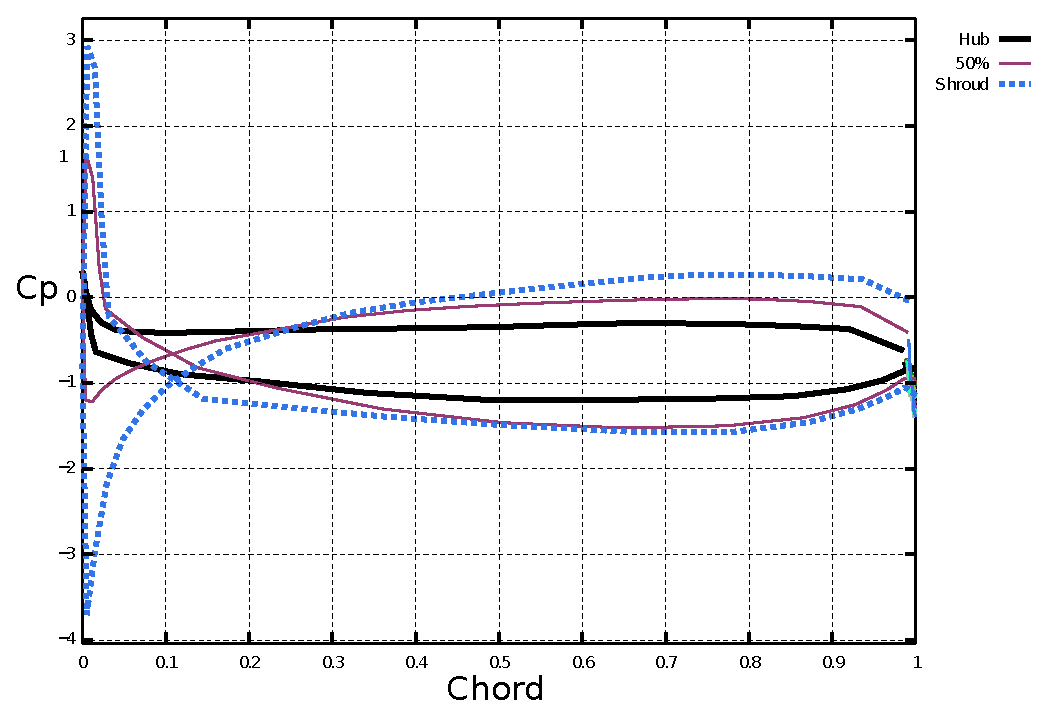
\includegraphics{pumps.eps}}
\end{minipage}
\caption{Pressure coefficient ($C_p$) distribution along the blade chordwise direction at part-load operation of a non-regulated hydraulic turbine at three spanwise locations: hub, mid-span and shroud. The pumping area corresponds to the first 10\% of the chord at mid-span and shroud locations}
\label{design-pumpS2}
\end{figure}

The partial pumping operation phenomenon can also be observed by the pressure coefficient ($C_p$) plots (fig.\ \ref{design-pumpS2}). The near-hub $C_p$ distribution (thick continuous line) is free from pumping areas. In contrast,  the near-shroud $C_p$ distribution (dashed line) suffers from partial pumping operation. The near-LE region of the shroud $C_p$ distribution exhibits the so-called ``crossed" distribution which denotes that the pressure at the pressure side of the blade is lower than that of the suction side. The thin continuous line is the mid-span $C_p$ distribution which suffers also from pumping operation, without however being as severe as close to the shroud.        
\FloatBarrier

\section{Optimization of a Francis Turbine Runner} % top level followed by section, subsection
The design-optimization of a Francis turbine runner is presented in this section. Due to the great number of design variables used to parameterize the candidate geometries, this case is perfectly suited to demonstrate the gain from the use  of the KBD method. 
\label{Francis-runners}
\subsection{Francis Turbine}
Nowadays, Francis turbines are the most frequently used water turbines since they can operate in a considerable part of the discharge-head diagram (fig.\ \ref{range}) \cite{papanto}. Francis is a reaction type water turbine, named after its developer James B. Francis. 

\begin{figure}[h!]
\centering
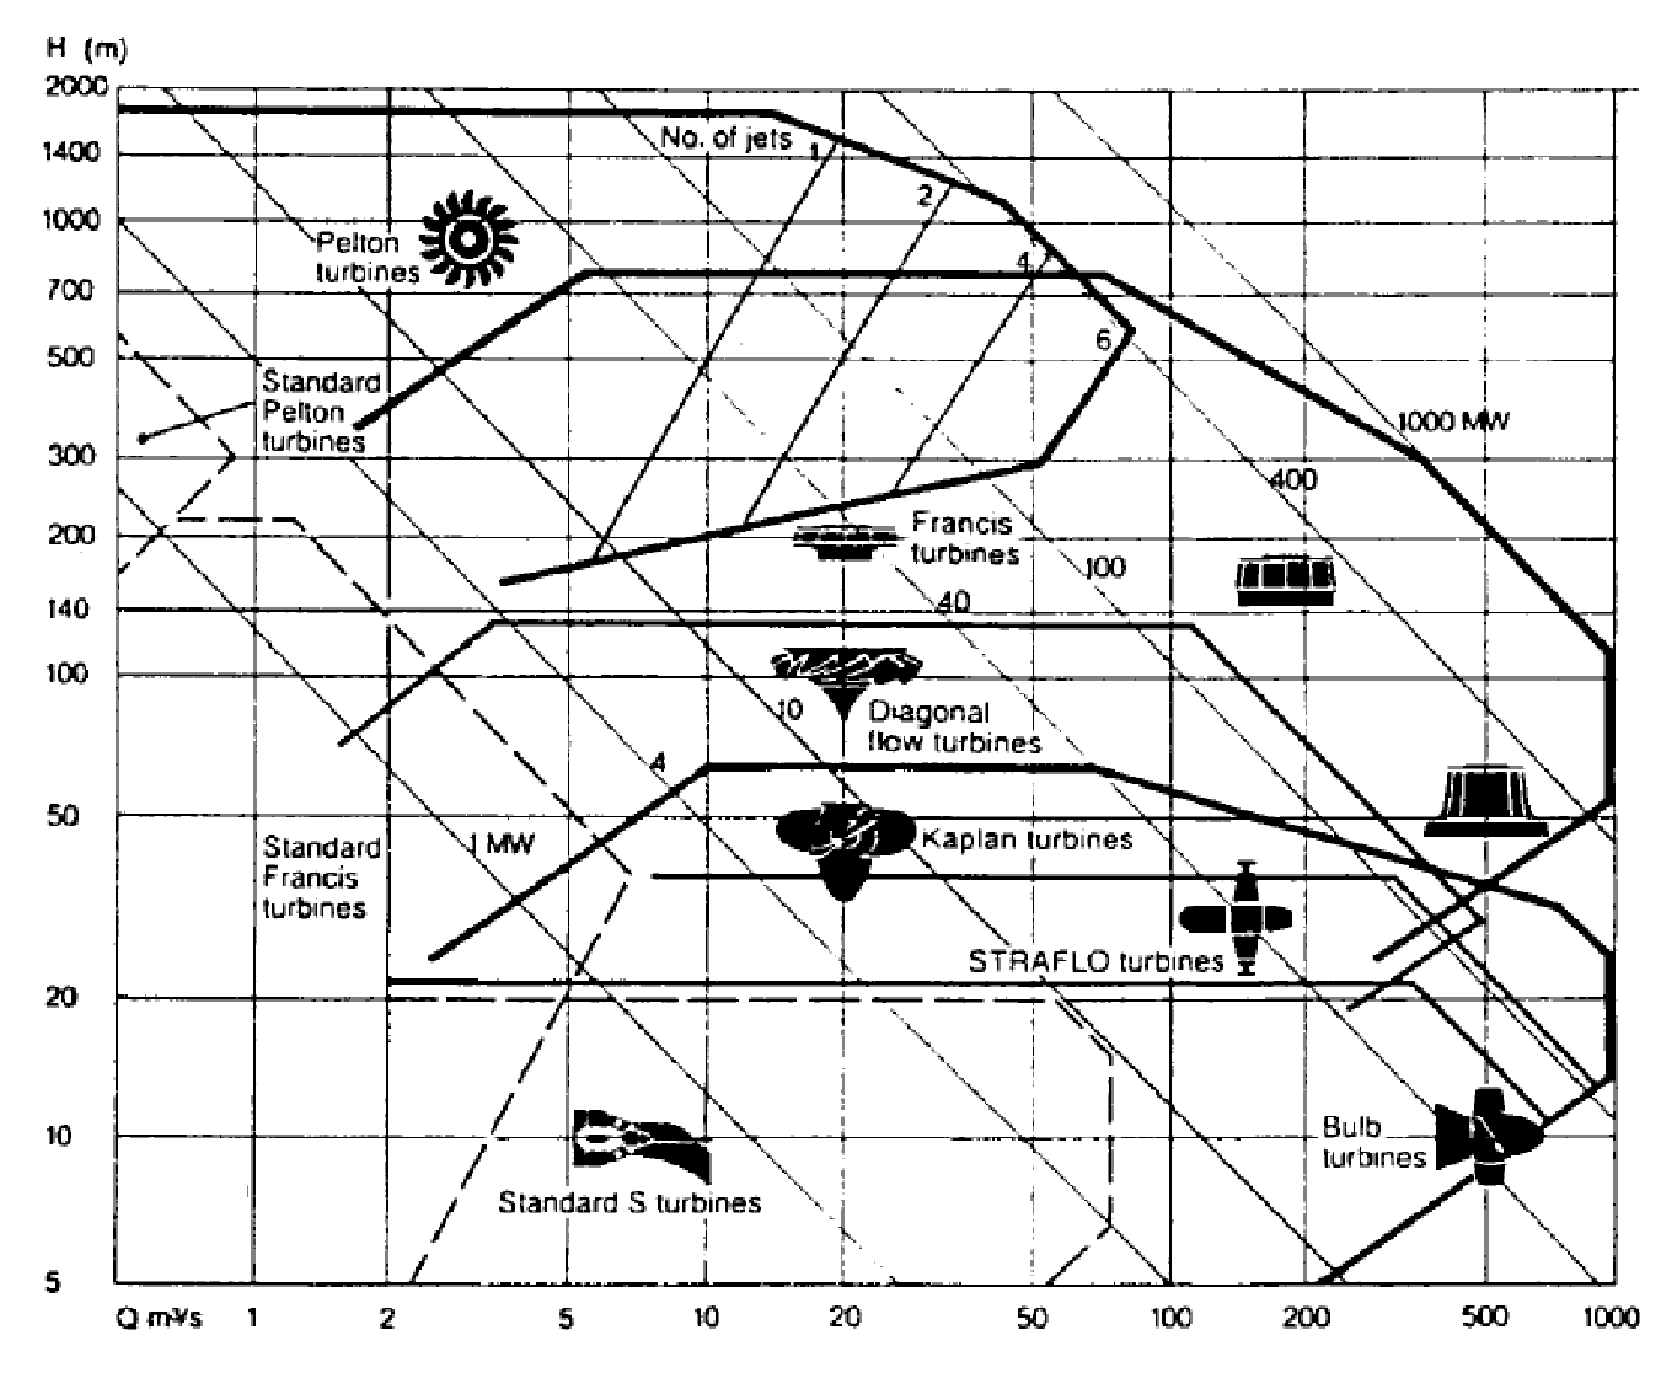
\includegraphics[width=140mm]{range2.eps} 
\caption{Range of application for the different turbine types, \cite{papanto}.}
\label{range}
\end{figure}

A typical Francis turbine consists of four parts (fig.\ \ref{francis1}). The spiral casing together with the stay-vanes are designed to provide uniform water intake along the entire circumference of the wicket-gates inlet. The wicket-gates (or guide-vanes) are adjustable to allow efficient turbine operation for a range of water flow conditions. The runner aims at harnessing the hydraulic energy. Finally, the draft-tube is used to transform the outlet kinetic energy into head.

\begin{figure}[h!]
\centering
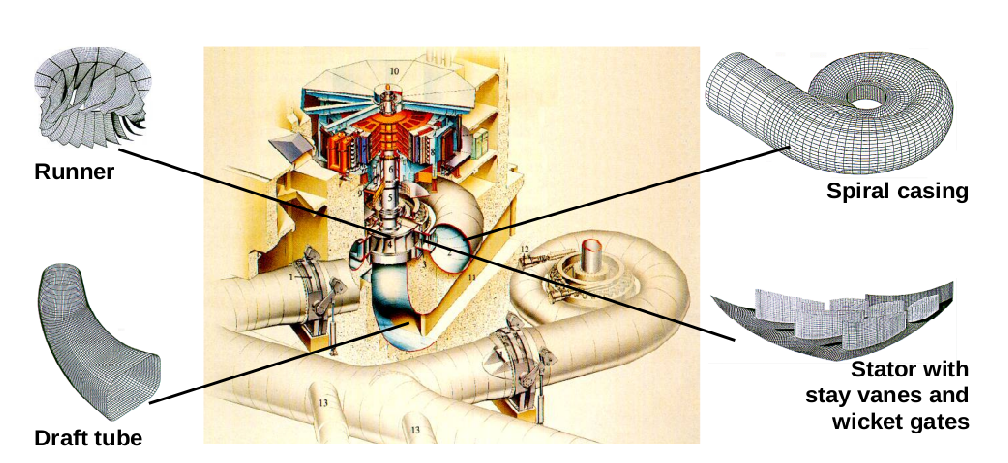
\includegraphics[width=150mm]{francis1.eps} 
\caption{Francis turbine and its constituent parts, \cite{andritz}.}
\label{francis1}
\end{figure}

\subsection{Case Presentation}
From the industrial point of view, the design problem in hand is referred to as a modernization/rehabilitation project, since it mainly aims at upgrading the runner (fig.\  \ref{design-parameterization}) for using it in an existing power plant. Modernization/rehabilitation projects are fairly common world-wide and, particularly in Europe where almost all large-hydro locations are already tapped and a lot of them are rather ``aged''. Typical reasons for modernization/rehabilitation project are:
\begin{itemize}
\item[\textbf{(a)}] to increase the reliability and availability of the power plant; 
\item[\textbf{(b)}] to extend its life and restore its performance; 
\item[\textbf{(c)}] to improve its performance, including:
\begin{itemize}
	\item efficiency and/or power,
    \item reduction of cavitation erosion,
	\item enlargement of the operating range,
\end{itemize}
\item[\textbf{(d)}] to improve plant safety;
\item[\textbf{(e)}] to resolve environmental, social or regulatory issues;
\item[\textbf{(f)}] to reduce the maintenance or operating cost;
\item[\textbf{(g)}] to take into account other parameters, such as:
\begin{itemize}
	\item modified governmental regulations,
	%\item political criteria;
	\item modified hydrology conditions or
	\item modified market conditions.
\end{itemize}
\end{itemize}

In modernization/rehabilitation projects, the designer must ensure that the newly designed runner fits perfectly in the pre-existing structure by respecting both geometrical and hydraulic-behaviour constraints. Geometrical constraints are mostly related to the inlet-outlet diameters and the hub-shroud meridional contour. On the other hand, the runner should respect given inlet flow conditions and also a new objective associated with the draft-tube coupling must be considered, in addition to those related to efficiency and cavitation. The reason is that, at the outlet, the runner must meet an existing draft-tube inlet which works optimally for a specific inlet velocity profile.      
  
\begin{figure}[h!]
\begin{minipage}[b]{1\linewidth}
 \centering
 \resizebox*{7cm}{!}{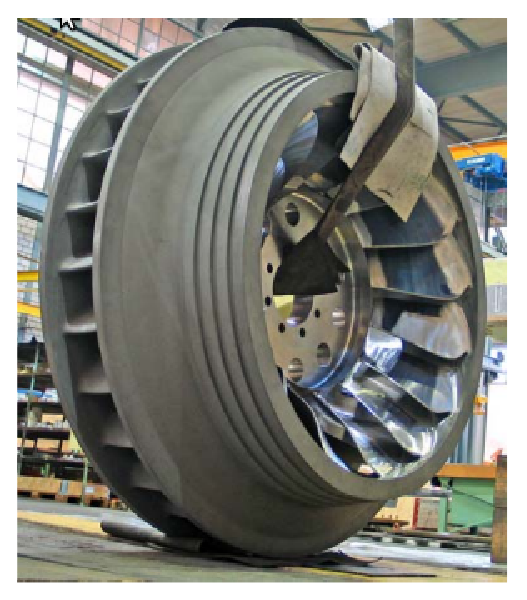
\includegraphics{francis2.eps}}
\end{minipage}
%\begin{minipage}[b]{0.5\linewidth}
% \centering
% \resizebox*{7.5cm}{!}{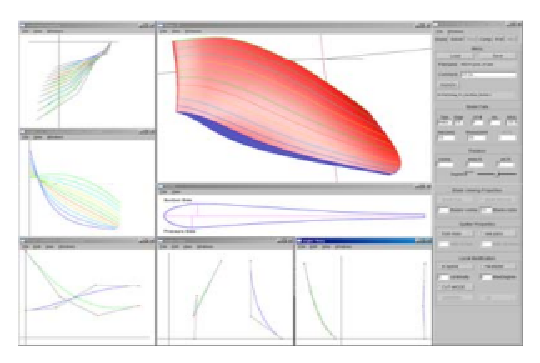
\includegraphics{francis3.eps}}
%\end{minipage}
\caption{Optimization of a Francis Turbine: An existing Francis runner, quite similar to the one designed herein, is shown, \cite{andritz}. }%Right; demonstration of Francis runner parameterization}
\label{design-parameterization}
\end{figure}

%\subsubsection{Case formulation}
%Herein the case formulation that transforms the above design case into a basic optimization problem will be presented. Given that the optimization problem definition is (cite EA chapter);
%\begin{align} 
%   &min ~ F(x)=(f_1(x),f_1(x),...,f_M(x))\in \Re^{M} \nonumber \\
%   &\mbox{subject to} ~ c_k(x)\leq d_k ~ k =1,K
%\label{Optim}
%\end{align}
%,where $x\in X \!\leq\! \Re^{N}$ is the design vector and $X$ the design space, $c(x)$ the constraints vector and $F(x)$ the objectives vector.

\subsubsection{Design Parameterization}
The design variables and their corresponding ranges are picked from the set specified in section \ref{Paramt} through a user-friendly graphical interface integrated in the parameterization tool, \cite{dipl_livia,dipl_simon}.  In this  case, the design vector consists of $336$ design variables, as in table \ref{design_vars}.


%\begin{figure}[h!]
%\begin{minipage}[b]{1\linewidth}
% \centering
% \resizebox*{7cm}{!}{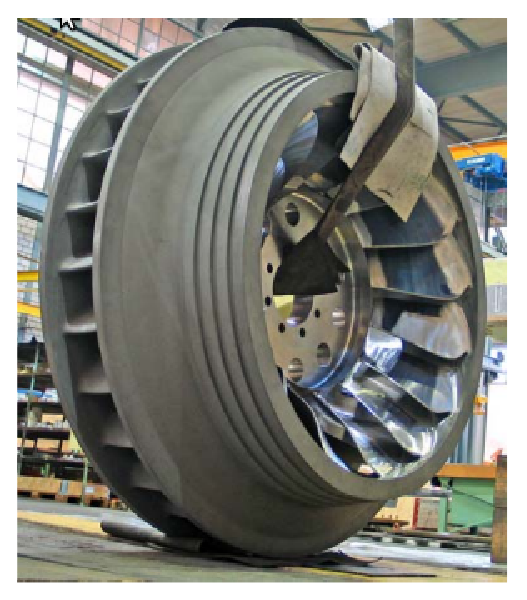
\includegraphics{francis2.eps}}
%\end{minipage}
%\begin{minipage}[b]{1\linewidth}
% \centering
% \resizebox*{14cm}{!}{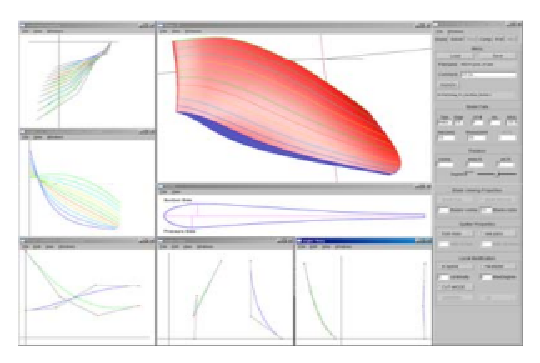
\includegraphics{francis3.eps}}
%\end{minipage}
%\caption{Optimization of a Francis Turbine: Graphical interface integrated in the parameterization tool.}
%\label{design-parameterization}
%\end{figure}


\begin{table}[h!]
\begin{center}
\begin{tabular}{ |c|l| }
\hline

Number of              & used to parameterize the:\\
design variables       & \\
\hline
6 & Spanwise distributions of $\theta_{LE}$\\
\hline
6 & Spanwise distributions of $\theta_{TE}$\\
\hline
6 & Spanwise distributions of $\beta_{LE}$\\
\hline
6 & Spanwise distributions of $\beta_{TE}$\\
\hline
6 & Spanwise distributions of $\zeta_{LE}$\\
\hline
6 & Spanwise distributions of $\zeta_{TE}$\\
\hline
6 & Spanwise thickness distributions for PS \\
\hline
6 & Spanwise thickness distributions for SS\\
\hline
8 & LE projection on the meridional plane\\
\hline
8 & TE projection on the meridional plane\\
\hline
4 & Shroud generatrix (on the meridional plane) \\
\hline
4 & Hub generatrix (on the meridional plane)\\
\hline
$12 \times 11$ & Airfoil profiles for the PS (11 profiles)\\
\hline
$12 \times 11$ & Airfoil profiles for the SS (11 profiles)\\
\hline
\hline
336 & Design variables, in total \\
\hline   
\end{tabular}
\caption{
The design variables used to parameterize the Francis runner.}
\label{design_vars}
\end{center}
\end{table}

%\begin{figure}[h!]
%\begin{minipage}[b]{1\linewidth}
% \centering
% \resizebox*{13cm}{!}{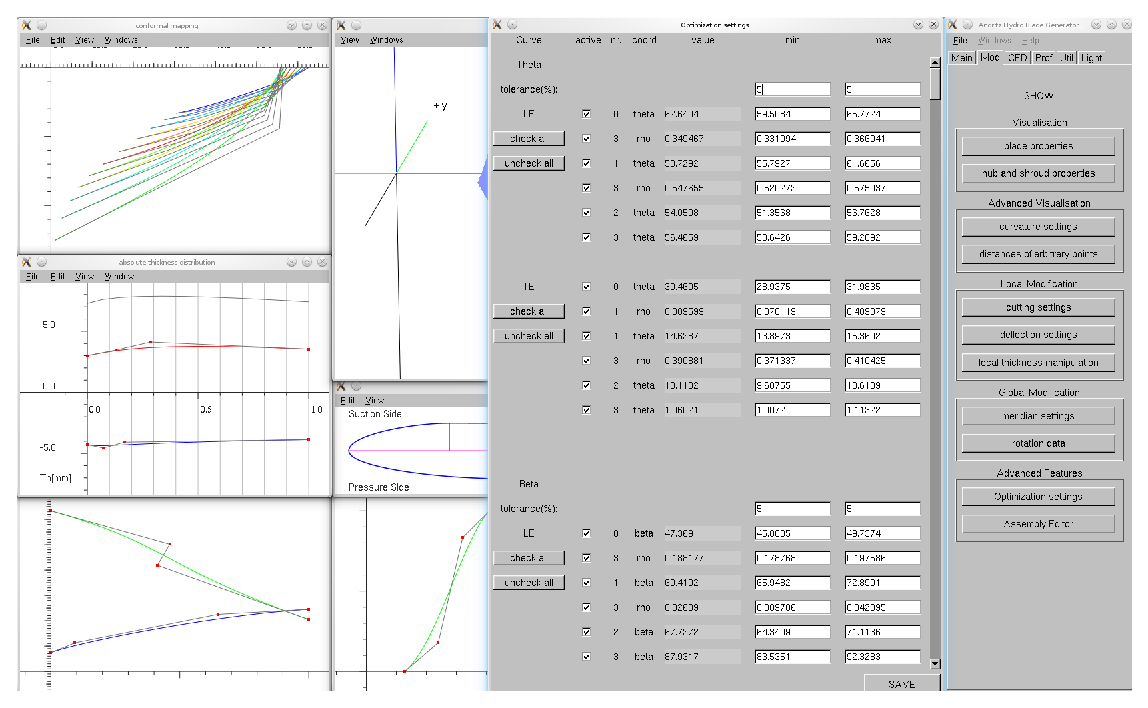
\includegraphics{pic2.eps}}
%\end{minipage}
%\caption{Optimization of a Francis Turbine: Graphical interface integrated in the parameterization tool.}
%\label{design-parameterization2}
%\end{figure}

\subsubsection{Objectives and Constraints}
The objective vector comprises of two objectives which correspond to the outlet velocity profile metric ($M_1$) and the blade loading quality one ($M_2$). To define $M_1$, the user-defined target profiles shown in fig.\ \ref{design-obj-tar} are used. 



\begin{figure}[h!]
\begin{minipage}[b]{1\linewidth}
 \centering
 \resizebox*{10.0cm}{!}{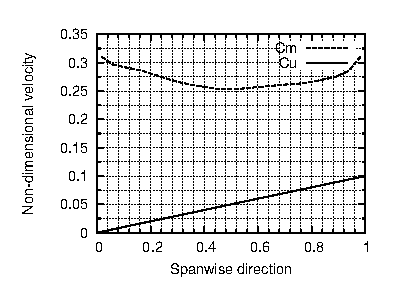
\includegraphics{Target.eps}}
\end{minipage}
\caption{Optimization of a Francis Turbine: Target non-dimensional velocity profile distributions at the runner-outlet.}
\label{design-obj-tar}
\end{figure}


To ensure performance stability, the runner to be designed is desirable to yield optimal performance at three operating points, the best efficiency (BE) point, the part-load (PL) and full-load (FL) ones. %(best efficiency point H=36m, part-load H=30m and full-load H = 43.5m). 
The three-operating-point design is handled as an optimization problem with two objectives, where the value of each objective function is computed for each operating point separately (eq. \ref{ObjFrancis}) and, then, the “overall” value $f_i$ is set equal to the weighted sum of the corresponding values for the three operating points, (table \ref{op-weights}). Thus, if


\begin{eqnarray}
   f_1^i=M_1^i ~~~,~~~ f_2^i=M_2^i 
   \label{ObjFrancis} 
\end{eqnarray}
where the superscript $i=1,2,3$ denotes the operating point, then
\begin{eqnarray}
   f_1=\sum^3_{i=1}w_if_1^i ~~~,~~~ f_2=\sum^3_{i=1}w_if_2^i 
   \label{ObjFrancis2} 
\end{eqnarray}
where $w_i$ the weights for each operating point (table \ref{op-weights}).


\begin{table}[h!]
\begin{center}
\begin{tabular}{ |c|l| }
\hline
Operating point& Weight $(w_i)$\\
\hline
Best Efficiency (BE), $i=1$ & 1.0\\
\hline
Part-Load (PL), $i=2$ & 0.3\\
\hline
Full-Load (FL), $i=3$ & 0.3\\
\hline
\end{tabular}
\caption{Optimization of a Francis Turbine: Operating point weights.}
\label{op-weights}
\end{center}
\end{table}


For each operating point, two constraints are imposed (table \ref{Cons}). The first is related to the cavitation safety and the second aims at ensuring that the turbine operates at the desired point. The cavitation constraint is based on the $\sigma_{Hist}$ method, as presented in section \ref{cav.metric}. Operating point control is carried out by imposing constraints on the maximum distance from the desired operating point. Here, given that the massflow is fixed due to the imposed inlet boundary conditions, the operating point is controlled via constraints imposed onto the hydraulic height 


\begin{eqnarray}
   \Delta H=\frac{H_{computed}-H_{desirable}}{H_{desirable}} 
   \label{ConstFrancis} 
\end{eqnarray}
where $H_{desirable}$ the height of the desirable operating point.

\begin{table}[h!]
\begin{center}
\begin{tabular}{ |c|c|c| }
\hline
Operating point & $\sigma_i^{Hist}<\sigma$ & Hydraulic height\\
\hline
BE & $\sigma_i^{Hist}<0.2$ & $|\Delta H^i|<1.5\%$\\
\hline
PL       & $\sigma_i^{Hist}<0.2$ & $|\Delta H^i|<5\%$\\
\hline
FL       & $\sigma_i^{Hist}<0.2$ & $|\Delta H^i|<5\%$\\
\hline
\end{tabular}
\caption{Optimization of a Francis Turbine: Constraints per operating point.}
\label{Cons}
\end{center}
\end{table}


%\begin{figure}[h!]
%\begin{minipage}[b]{0.5\linewidth}
% \centering
% \resizebox*{7.0cm}{!}{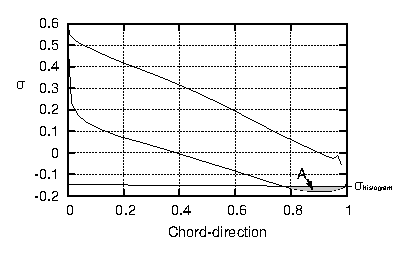
\includegraphics{sigma.eps}}
%\end{minipage}
%\begin{minipage}[b]{1\linewidth}
% \centering
% \resizebox*{10.0cm}{!}{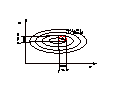
\includegraphics{con1.eps}}
%\end{minipage}
%\caption{Optimization of a Francis Turbine: Maximum distance from %operating point equals to $\pm2\%$.}
%\label{design-obj3}
%\end{figure}

\subsection{Results}
As mentioned above, this case is used to demonstrate the use of the proposed KBD method in industrial environment. Therefore, two optimization procedures were tried: one by using the conventional EA since the large number of design variables makes the use of metamodels (as in standard MAEA) inefficient and a second one using the KBD-MAEA method.

\subsubsection{Archived Designs}
Three archived designs were available (fig.\ \ref{design-bases}). These designs were developed to perform optimally at operating points close to those set for the desired blade. The criteria used to find relevant archived designs were the non-dimensional specific speed $N_{ED}$ and specific massflow $Q_{ED}$ \footnote{$N_{ED}$ and $Q_{ED}$ are dimensionless quantities based on energy (E=1) and diameter (D=1) used to characterize turbine operation.} defined as follows 

\begin{eqnarray}
   N_{ED}=\frac{n}{60}\frac{D}{\sqrt{gH}}, ~~~~~~ Q_{ED}=\frac{Q}{D^2 \sqrt{gH}}
   \label{undimFrancis} 
\end{eqnarray}

%Since those design were fitted with their own, power plan specific, hub and shroud contours and given that during the modernization/rehabilitation project in hand. Those contours was asked to remain similar to the initial blade, some modifications were required in order to transform the archived designs into compatible with the required hub and shroud contours limitations. These modifications were restricted to simple stretching and pruning, something that requires practically zero time for the designer. However, as will be shown later in this section, this leads to designs with questionable quality. Nevertheless, this designs, with out any further hand-made refinements, are sufficient to be used as basis vectors in the KBD method.                           

\begin{figure}[h!]
\begin{minipage}[b]{1\linewidth}
 \centering
 \resizebox*{10.0cm}{!}{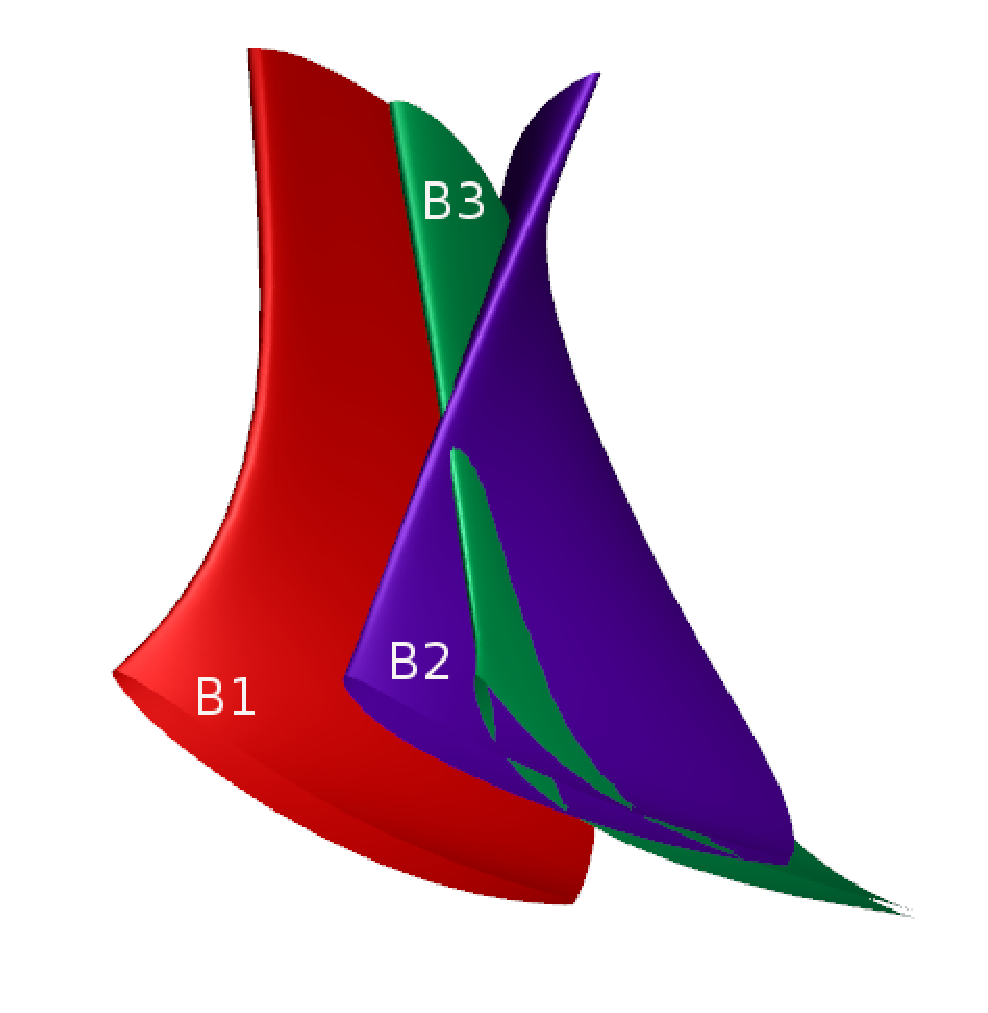
\includegraphics{Francis_bases.eps}}
\end{minipage}
\caption{Optimization of a Francis Turbine: The three archived geometries used as basis vectors.}
\label{design-bases}
\end{figure}

The archived designs to be used as basis vectors for this case were re-evaluated at the desirable operating points and their quality metrics are summarized in table \ref{reuse}.

\begin{table}[h!]
\begin{center}
\begin{tabular}{ |c|c|c|c|c|c| }
\hline
Archived & OP & $M_1$ & $M_2$  & $\sigma_i^{Hist}$ & $|\Delta H|$\\
Design &&&&&\\
\hline
 & BE & $0.472$ & $0.538$ & $0.21 > 0.2$ * & $ 5\% >1.5\%$ * \\
B1 & PL & $0.552$ & $0.824$ & $0.23 > 0.2$ * & $ 3.6\% <5\%$ \\
& FL & $0.408$ & $0.594$ & $0.2 = 0.2$  & $ 5.7\% >5\%$ * \\
\hline
\hline
& BE & $0.563$ & $0.922$ & $0.22 > 0.2$ * & $ 3.8\% >1.5\%$ * \\
B2 & PL & $0.534$ & $0.888$ & $0.24 > 0.2$ * & $ 2.6\% <5\%$  \\
& FL & $0.522$ & $1.178$ & $0.22 > 0.2$ * & $ 4.8\% <5\%$  \\
\hline
\hline
& BE & $0.402$ & $0.663$ & $0.19 < 0.2$  & $ 6.8\% >1.5\%$ * \\
B3 & PL & $0.515$ & $0.808$ & $0.21 > 0.2$ * & $ 6.9\% >5\%$ * \\
& FL & $0.257$ & $0.896$ & $0.18 < 0.2$  & $ 7.1\% >5\%$ * \\
\hline
\end{tabular}
\caption{Optimization of a Francis Turbine: Quality metrics (objectives and constraints) for the 3 archived designs (B1, B2 and B3) for all operating points (BE, PL and FL). An asterisk (*) next to an inequality means that the corresponding constraint is violated}
\label{reuse}
\end{center}
\end{table}

A closer look at B1 reveals the findings tabulated in table \ref{reuse}. For instance, from fig.\ \ref{Francis-B1-BE}, where $C_p$ iso-areas are plotted over the runner surfaces, areas which are prone to cavitation can be identified. From this figure, one may observe the lowest value of $C_p \!= \!-0.216$ which advocates the presence of cavitation, since $\sigma_i \! \approx \! -C_p \!= \!0.216$  . Recall that $\sigma \! = \! 0.2$ and that $\sigma_i$ must be greater than $\sigma$ for cavitation to appear. The $\sigma_i^{Hist}$ value which is equal to $0.21$, confirms this observation. Recall that $\sigma_i^{Hist}$ is a better estimation of $\sigma_i$ than the $-C_p$ one. So, the archived design B1 is suffering from cavitation even at the BE point. Fig. \ref{Francis-B1-BE} shows that regions with low $C_p$ which are prone to cavitation exist over the SS, near the TE, between mid-span and shroud. The archived design B1 suffers from cavitation at the PL point too and is just marginally safe at the FL  point (table \ref{reuse}). 

\begin{figure}[h!]
\begin{minipage}[b]{1\linewidth}
 \centering
 \resizebox*{14.0cm}{!}{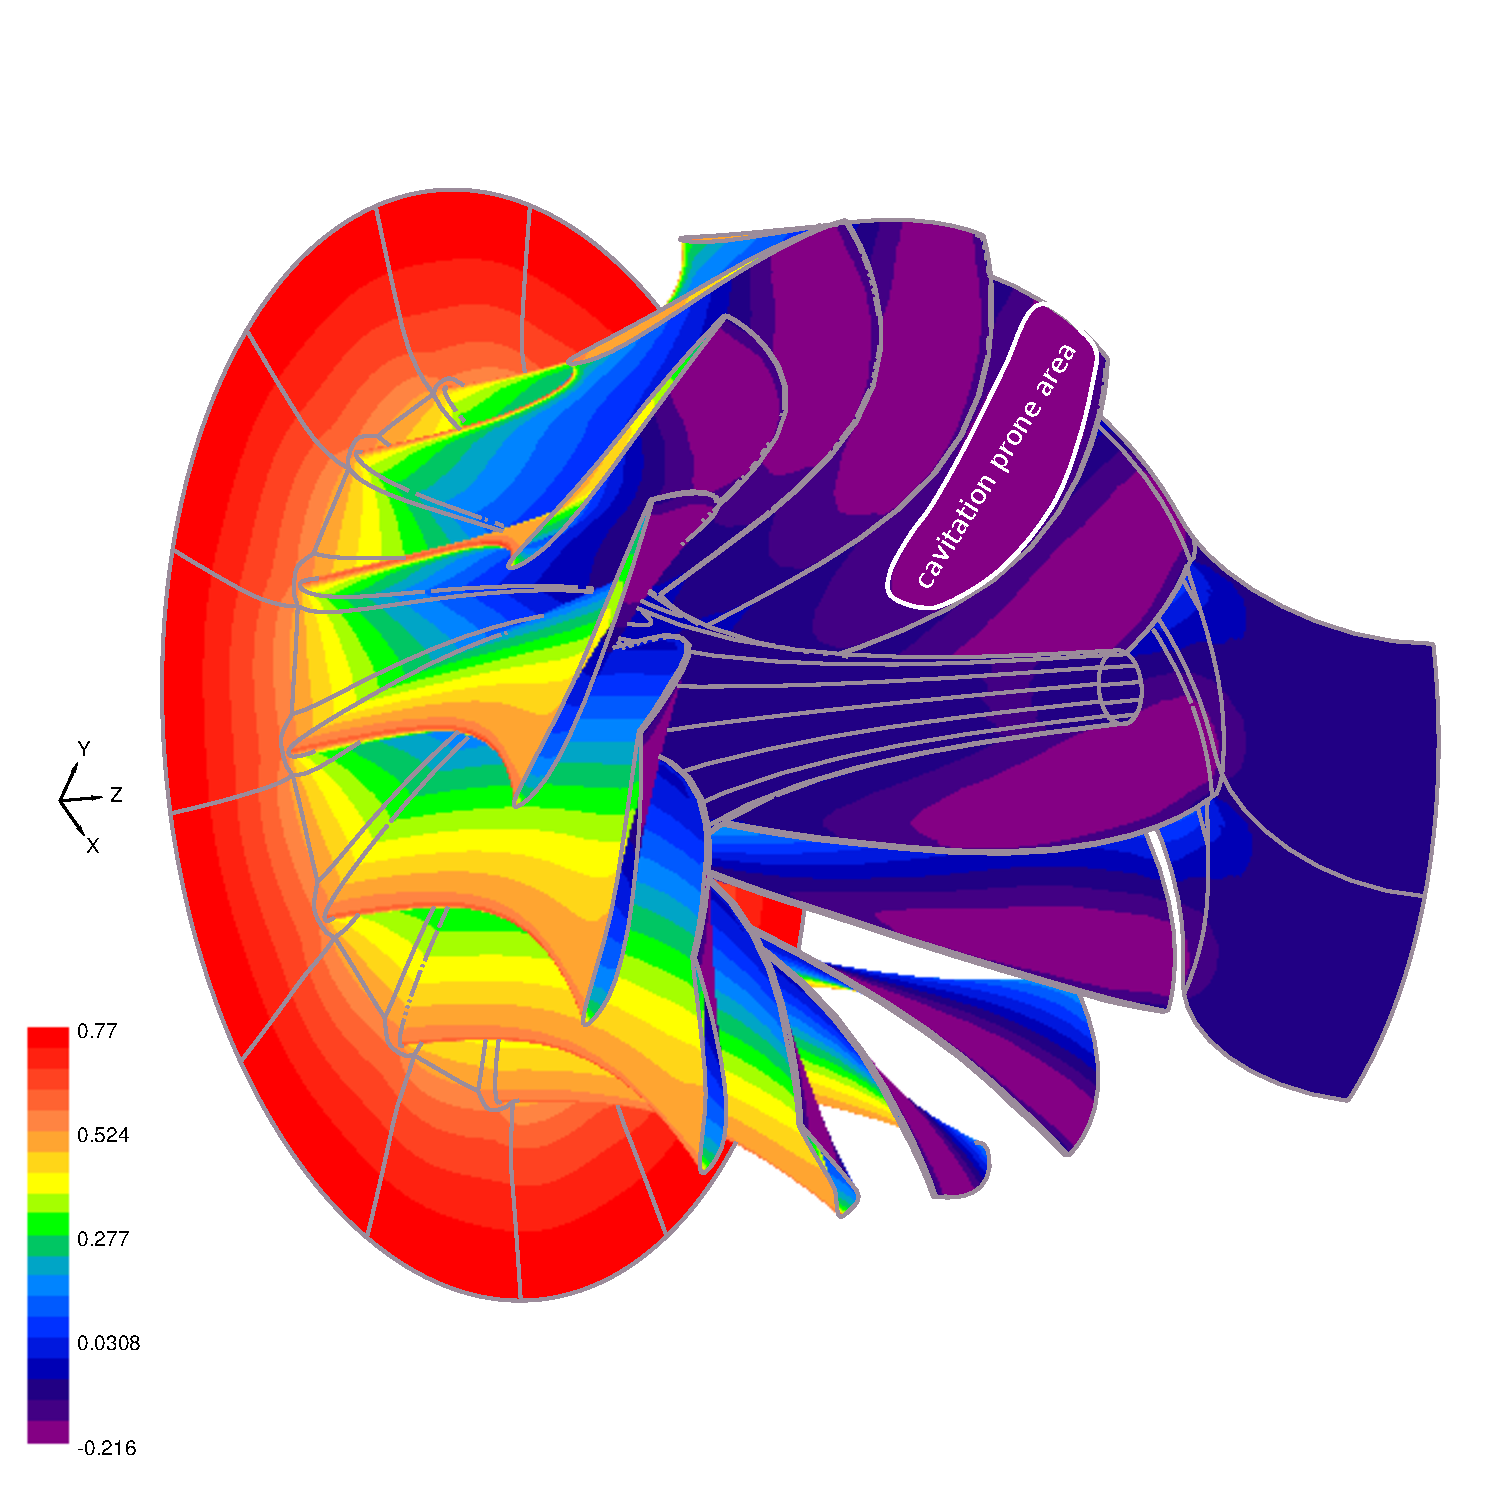
\includegraphics{B1.eps}}
\end{minipage}
\caption{Optimization of a Francis Turbine: $C_p$ iso-areas for the archived geometry B1, at the BE operating point. The area which is prone to cavitation (region with low $C_p$) is clearly marked at the SS, near the trailing edge, between mid-span and shroud.}
\label{Francis-B1-BE}
\end{figure}

Regarding the same design  B1, fig.\ \ref{Francis-B1-OUT} shows the noticeable deviation from the desirable outlet $C_m$ and $C_u$ velocity profiles for operating at BE point.  Dashed lines represent $C_m$ and continuous lines $C_u$. For the purpose of comparison, in the same plot, the target distributions are plotted with thicker lines.   

\begin{figure}[h!]
\begin{minipage}[b]{1\linewidth}
 \centering
 \resizebox*{11.0cm}{!}{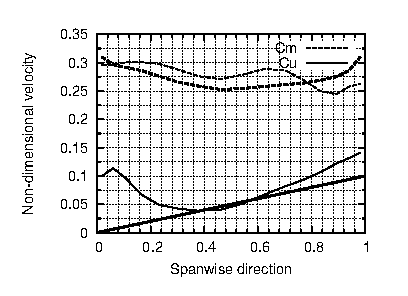
\includegraphics{OUTLET_B1.eps}}
\end{minipage}
\caption{Optimization of a Francis Turbine: $C_m$ and $C_u$ profiles for the archived design B1, operating at the BE point. The target distributions are plotted with thicker lines.}
\label{Francis-B1-OUT}
\end{figure}

The loading quality of B1 can be demonstrated through the chord-wise $C_p$ distribution plot, as defined in eq.\ \ref{Cpdef}, along the hub, mid-span and shroud (fig.\ \ref{Francis-B1-LOAD}). Though, at mid-span and hub, relatively good loading behaviour is observed, the blade part which is close to the shroud suffers from important load differences.      

\begin{figure}[h!]
\begin{minipage}[b]{1\linewidth}
 \centering
 \resizebox*{11.0cm}{!}{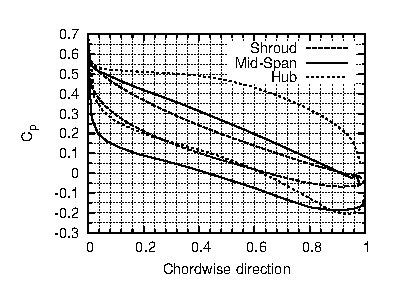
\includegraphics{Load_B1.eps}}
\end{minipage}
\caption{Optimization of a Francis Turbine: $C_p$ profiles hub, mid-span and shroud for the archived design B1, for the BE operating point.}
\label{Francis-B1-LOAD}
\end{figure}

\FloatBarrier
Regarding B2, the existing blade suffers from cavitation at all three operating points, see table \ref{reuse}. Fig.\ \ref{Francis-B2-BE} shows the $C_p$ iso-areas over the runner blade surface of B2, operating at the BE point. The lower limit of $C_p$, $(C_p\!=\!-0.234)$ denotes that it is likely for cavitation to appear and this is confirmed by the computed $\sigma_i^{Hist}$ values (table \ref{reuse}). Fig.\ \ref{Francis-B2-BE} shows that cavitation occurs over the suction side near the trailing edge at the near hub region.     


\begin{figure}[h!]
\begin{minipage}[b]{1\linewidth}
 \centering
 \resizebox*{14.0cm}{!}{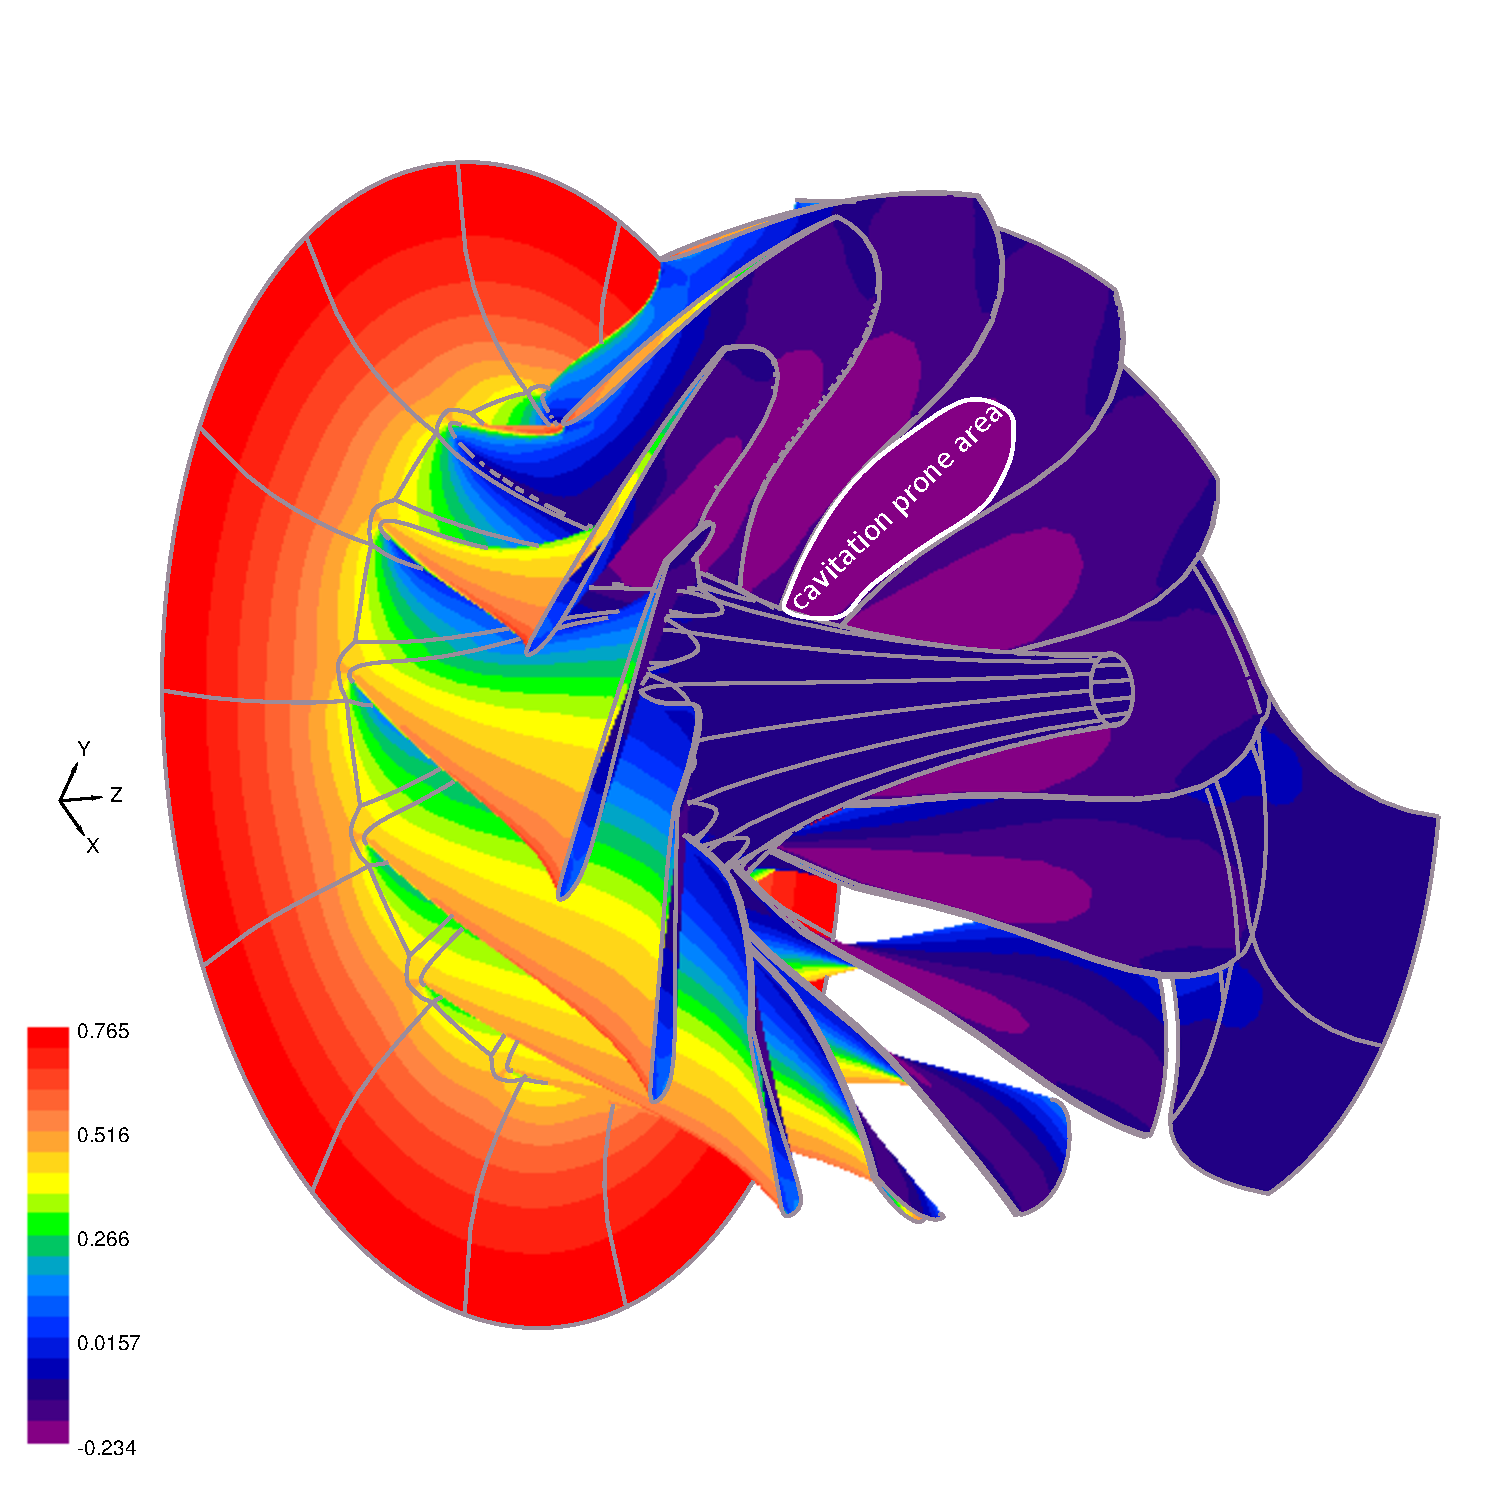
\includegraphics{B2.eps}} %Pics located at /home/stelios/Desktop/BEMPOSTA/MAEA_CBR_case_Bemposta_4/Bases/
\end{minipage}
\caption{Optimization of a Francis Turbine: $C_p$ iso-areas for the archived design B2 operating at the BE point. Cavitation occurs on the SS, near the TE close to the hub.}
\label{Francis-B2-BE}
\end{figure}

The outlet velocity quality is plotted in fig. \ref{Francis-B2-OUT}. $C_m$ is far away from the desirable distribution and $C_u$, close to the hub, has locally high values.   

\begin{figure}[h!]
\begin{minipage}[b]{1\linewidth}
 \centering
 \resizebox*{11.0cm}{!}{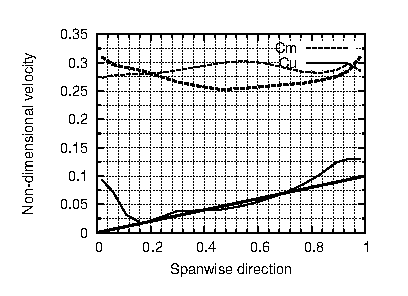
\includegraphics{OUTLET_B2.eps}}
\end{minipage}
\caption{Optimization of a Francis Turbine: $C_m$ and $C_u$ profiles for the archived design B2 at the BE operating point. The target distributions are plotted with thicker lines.}
\label{Francis-B2-OUT}
\end{figure}

From the $C_p$ profiles computed for the archived design B2 operating at the BE point (fig. \ref{Francis-B2-LOAD}), one may observe the non-satisfactory loading quality; the same information can be obtained from table \ref{reuse}. In the three spanwise positions, there are important load differences along the chord direction. 

\begin{figure}[h!]
\begin{minipage}[b]{1\linewidth}
 \centering
 \resizebox*{11.0cm}{!}{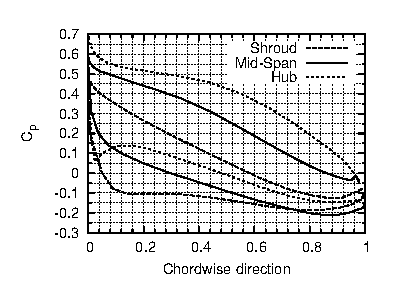
\includegraphics{Load_B2.eps}}
\end{minipage}
\caption{Optimization of a Francis Turbine: $C_p$ profiles at hub, mid-span and shroud for archived design B2 at the BE point.}
\label{Francis-B2-LOAD}
\end{figure}

\FloatBarrier
Archived design B3 is clean from cavitation at all but the PL operating point, see table \ref{reuse}. Fig.\ \ref{Francis-B3-PL} shows the $C_p$ iso-areas for  B3 operating at the PL point. The lowest $C_p$ value observed, namely $C_p= -0.215$, is a clear indication of the presence of cavitation, as also confirmed by the computed $\sigma_i^{Hist}$ value (table \ref{reuse}). Cavitation is observed at the suction side near the TE.     


\begin{figure}[h!]
\begin{minipage}[b]{1\linewidth}
 \centering
 \resizebox*{14.0cm}{!}{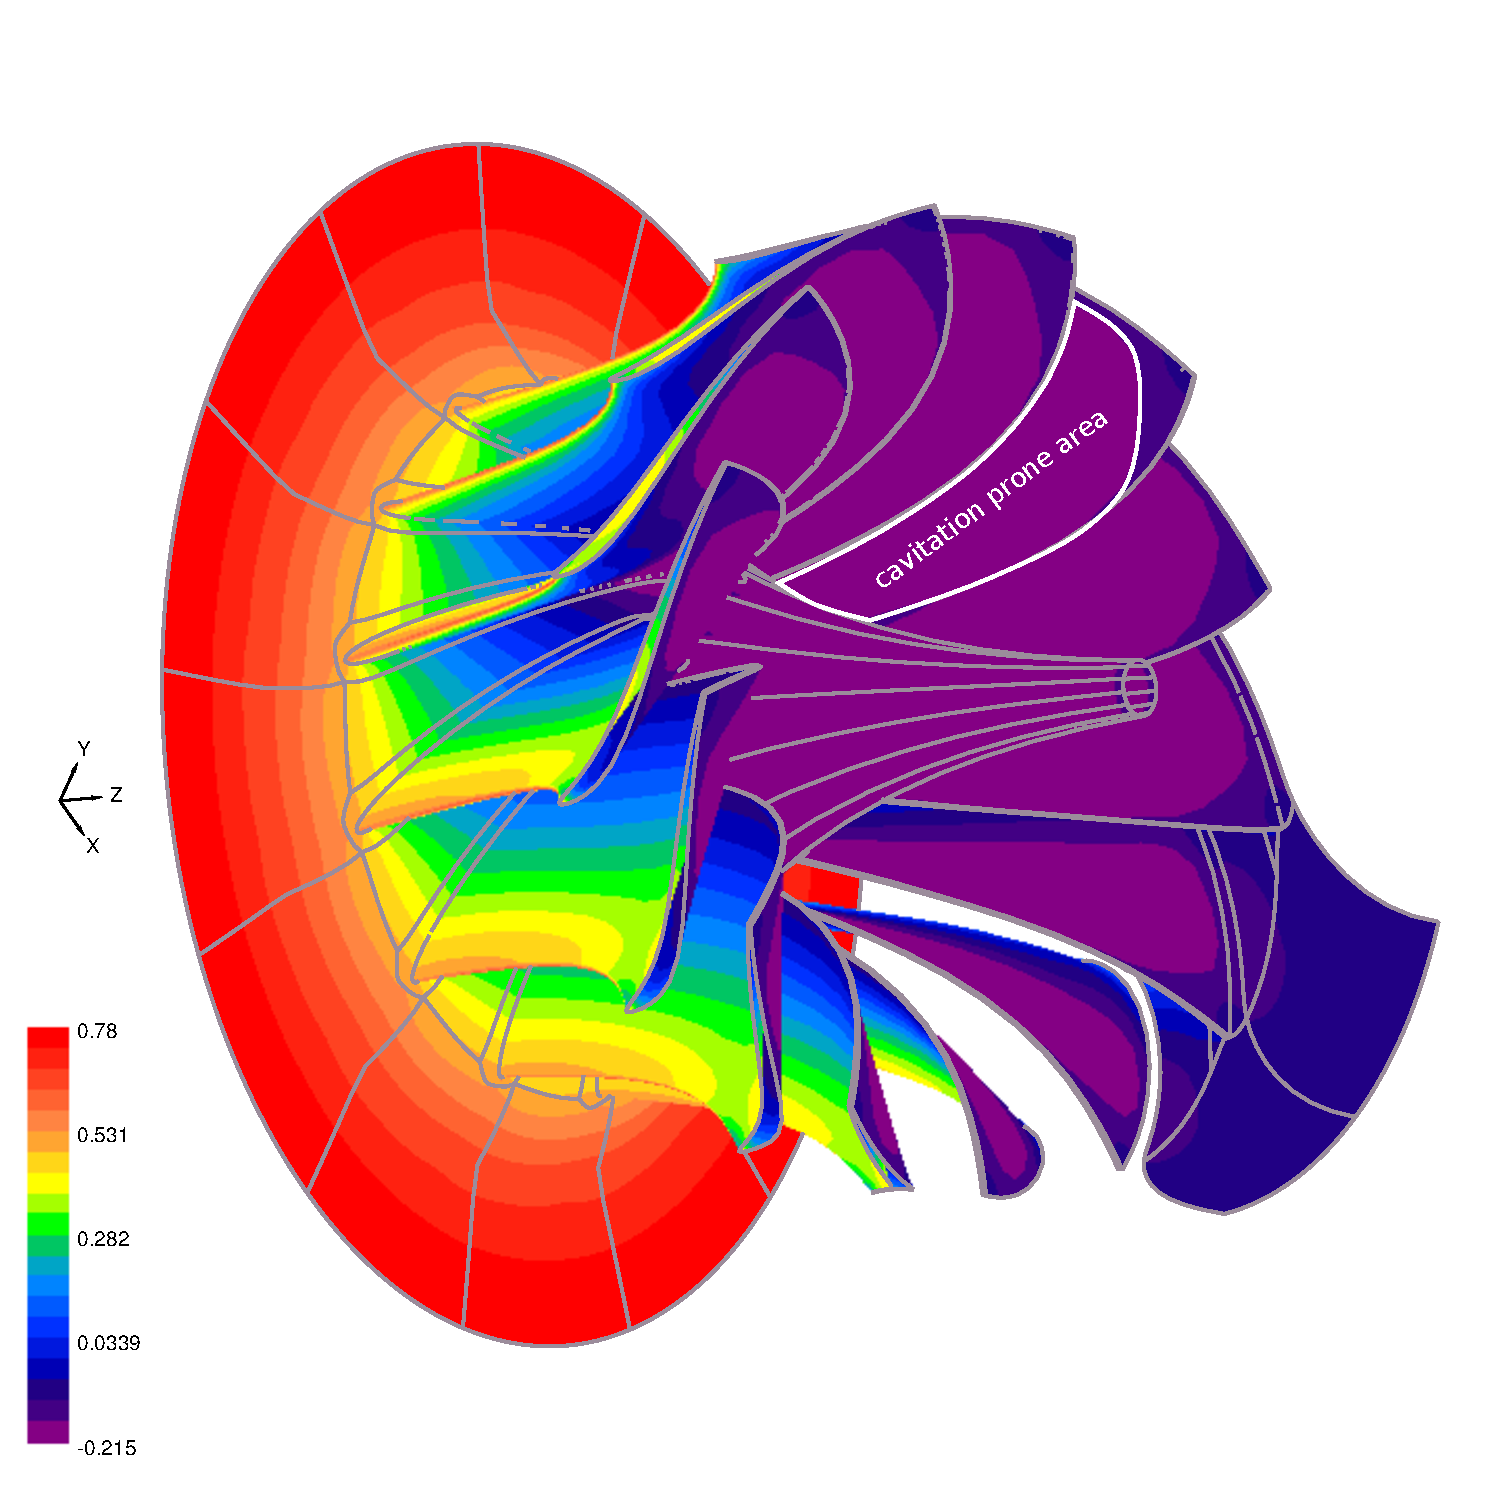
\includegraphics{B3.eps}}
\end{minipage}
\caption{Optimization of a Francis Turbine: $C_p$ iso-areas for archived design B3 at PL operating point. Cavitation is observed at the SS near the TE.}
\label{Francis-B3-PL}
\end{figure}

Regarding the outlet velocity profile quality, fig.\ \ref{Francis-B3-OUT}, both $C_m$  and $C_u$ deviate considerably from the desirable distributions.   

\begin{figure}[h!]
\begin{minipage}[b]{1\linewidth}
 \centering
 \resizebox*{11.0cm}{!}{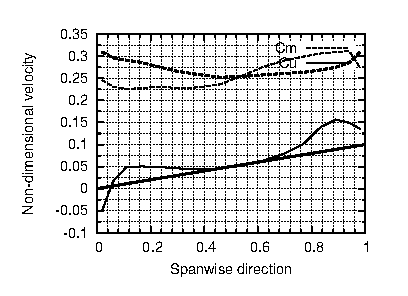
\includegraphics{OUTLET_B3.eps}}
\end{minipage}
\caption{Optimization of a Francis Turbine: $C_m$ and $C_u$ profiles for the archived design B3, at the BE point. For the purpose of comparison, in the same plot the target distributions are plotted with thicker lines.}
\label{Francis-B3-OUT}
\end{figure}

Loading quality is demonstrated in fig.\ \ref{Francis-B3-LOAD}. The computed $C_p$ profile at the shroud shows important loading differences. 

\begin{figure}[h!]
\begin{minipage}[b]{1\linewidth}
 \centering
 \resizebox*{11.0cm}{!}{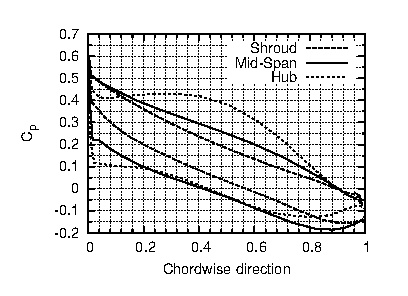
\includegraphics{Load_B3.eps}}
\end{minipage}
\caption{Optimization of a Francis Turbine: $C_p$ profiles hub, mid-span and shroud, for the archived design B3, at the BE point.}
\label{Francis-B3-LOAD}
\end{figure}

Since none of the three archived designs shows ``good'' outlet velocity profiles and loading and, also, doesn't respect the imposed constraints, a ``Revise'' step is needed. In this thesis, this step is based on EAs, with or without metamodels. So, practically, two optimizations have been carried out. The first was based on a conventional EA ($\mu\!=\!30,\lambda\!=\!120$) using $336$ design variables, according to the aforementioned parameterization. The second employed the proposed KBD method, i.e. the so-called KBD-MAEA ($\mu\!=\!20,\lambda\!=\!60,\lambda_e\!=\! 4\! ~\! to\!~\! 8$, with the IPE phase starting after recording the first $150$ non-failed individuals in the DB). The KBD-MAEA run handled $19$ optimization variables. For both optimizations, the three archived designs were injected in the population of the first generation.

Regarding KBD, the $19$ optimization variables result from grouping the design variables (eq. \ref{non-linear2}) into $6$ groups (table \ref{design_groups}) plus the extrapolation variable $\Psi$. This set-up requires $6$ weights to control the influence of each one of the archived designs to any candidate solution, giving rise to $18$ weights, in total.

\begin{table}[h!]
\begin{center}
\begin{tabular}{ |c|l| }
\hline

Group              & Design variables determining the:\\
\hline
1 & Spanwise distributions of $\theta_{LE}$\\
\hline
1 & Spanwise distributions of $\theta_{TE}$\\
\hline
2 & Spanwise distributions of $\beta_{LE}$\\
\hline
2 & Spanwise distributions of $\beta_{TE}$\\
\hline
3 & Spanwise distributions of $\zeta_{LE}$\\
\hline
3 & Spanwise distributions of $\zeta_{TE}$\\
\hline
4 & Spanwise thickness distributions for PS \\
\hline
4 & Spanwise thickness distributions for SS\\
\hline
5 & LE meridional position\\
\hline
5 & TE meridional position\\
\hline
5 & Shroud meridional generatrices \\
\hline
5 & Hub meridional generatrices\\
\hline
6 & Airfoil profiles for the PS (11 profiles)\\
\hline
6 & Airfoil profiles  for the SS (11 profiles)\\
\hline
\hline
6 & Groups, in total \\
\hline   
\end{tabular}
\caption{
Optimization of a Francis Turbine: The $6$ Groups  defining the $6 \times 3=18$ optimization variables out of the $19$ used in the KBD method.}
\label{design_groups}
\end{center}
\end{table}

The comparison of the performance of EA and KBD-MAEA is made using the hypervolume indicator \cite{Zitz2007}. The hypervolume indicator assumes that the quality of a Pareto front can be expressed by a scalar value which stands for the area or volume or hypervolume of the dominated, by the Pareto front, part of the objective space up to a user-defined nadir point. With the same nadir point, the higher the hypervolume indicator, the higher the quality of the Pareto front.

The comparison of the evolution of the hypervolume indicator in terms of the number of exact evaluations carried out by the EA and the KBD-MAEA is shown in fig.\ \ref{Francis-Res}. The horizontal axis expresses the CPU cost, by just making the realistic assumption that all evaluations have the same cost. 

\begin{figure}[h!]
\begin{minipage}[b]{1\linewidth}
 \centering
 \resizebox*{12.0cm}{!}{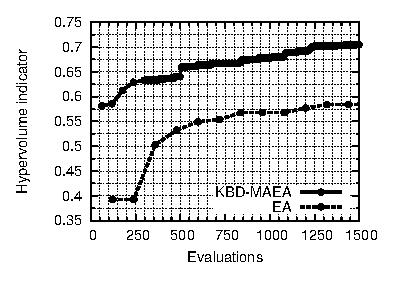
\includegraphics{HypComp.eps}}
\end{minipage}
\caption{Optimization of a Francis Turbine: hypervolume comparison between EA and the proposed KBD-MAEA method.}
\label{Francis-Res}
\end{figure}

The KBD-MAEA significantly outperforms the conventional EA. It starts with significantly better individuals in the first generation which demonstrates that, even though the archived designs are far from the optimal design, the grouping of the design variables and the use of normal distribution to set the importance regions in the design space are very close to the  ``physics'' of the problem in hand.    

\begin{figure}[h!]
\begin{minipage}[b]{1\linewidth}
 \centering
 \resizebox*{13.0cm}{!}{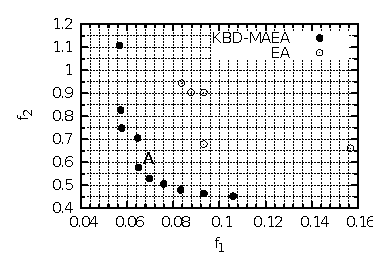
\includegraphics{Comp.eps}}
\end{minipage}
\caption{Optimization of a Francis Turbine: Fronts of non-dominated solutions computed at the cost of $1500$ exact evaluations by the EA and KBD-MAEA method. Optimal solution A was selected for further analysis (see figs.\ \ref{design-bases-a} to \ref{Francis-A-LOAD}).}
\label{Francis-Res-par}
\end{figure}

By examining fronts of non-dominated solutions (fig.\ \ref{Francis-Res-par}), as computed by the two methods at the same CPU cost of $1500$ exact evaluations, it can easily be concluded that designs of higher quality are obtained by the KBD-MAEA run. 
One of the non-dominated solutions computed by the KBD-MAEA, i.e. the one marked with A, was chosen for further analysis at the three operating points.


\begin{figure}[h!]
\begin{minipage}[b]{1\linewidth}
 \centering
 \resizebox*{12.0cm}{!}{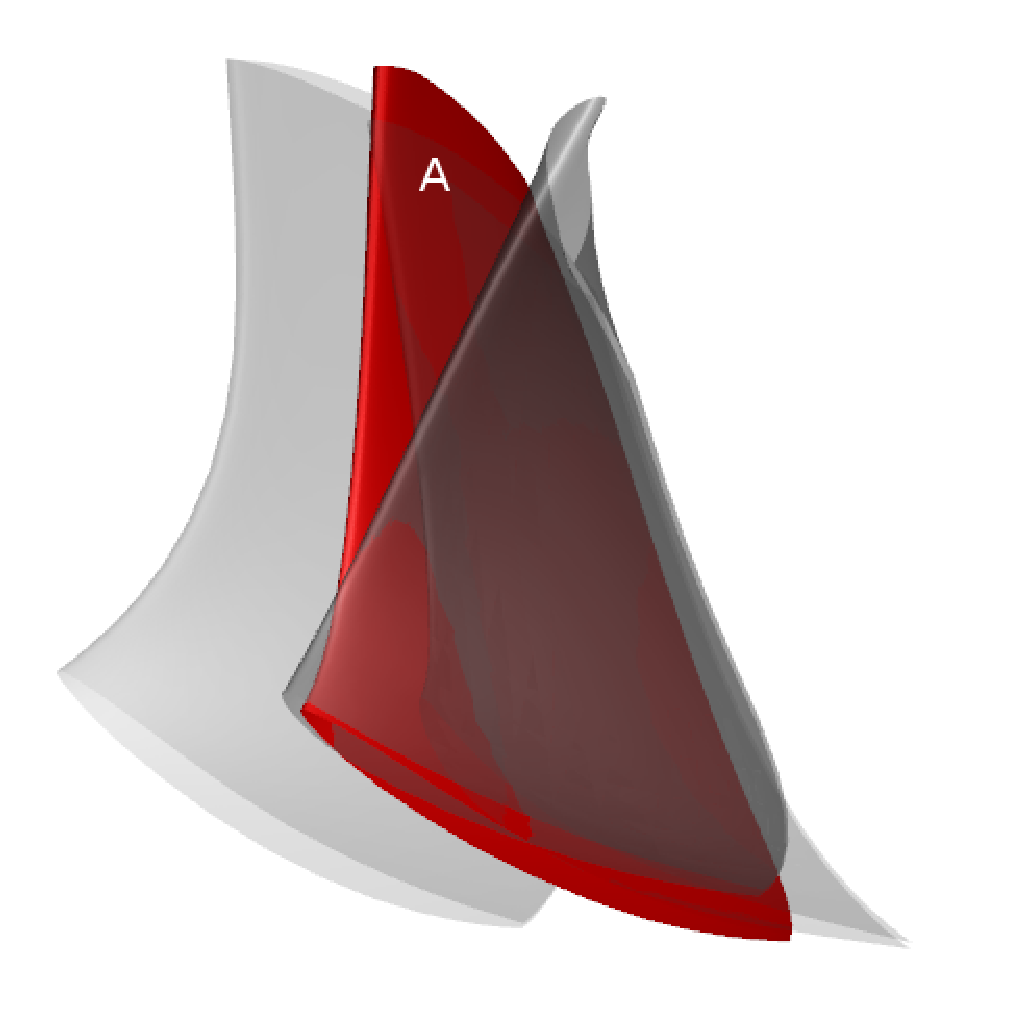
\includegraphics{final.eps}}
\end{minipage}
\caption{Optimization of a Francis Turbine: Design A and the three archived designs used. The high diversity among the four designs can be observed. The ability of the KBD method to produce designs, highly diversed in comparison with the archived ones is noticeable.}
\label{design-bases-a}
\end{figure}

The quality metrics of design A are summarized in table \ref{Asum}. To compare design A with the archived ones, its metrics should be compared with the values presented in table \ref{reuse}. This comparison reveals that, design A is significantly better that the three archived designs at all operating points and for both objectives. Design A is, in fact, a high quality blade.


\begin{table}[h!]
\begin{center}
\begin{tabular}{ |c|c|c|c|c|c| }
\hline
Geometry & OP & $M_1$ & $M_2$  & $\sigma_i^{Hist}$ & $|\delta H|$\\
\hline
& BE & $0.001$ & $0.302$ & $0.18 < 0.2$ & $ 1.1\% <1.5\%$ \\
A & PL & $0.086$ & $0.409$ & $0.19 < 0.2$ & $ 1.5\% <5\%$ \\
& FL & $0.092$ & $0.504$ & $0.18 < 0.2$ & $ 4.1\% <5\%$  \\
\hline
\end{tabular}
\caption{Optimization of a Francis Turbine: Quality metrics (objectives and constraints) regarding the chosen design A for all operating points (BE, PL $\&$ FL). The design is safe from cavitation at all operating points and operates within the desirable range.}
\label{Asum}
\end{center}
\end{table} 

Regarding cavitation, the behaviour of the selected design A can be seen by examining figs.\          \ref{Francis-A-BE}, \ref{Francis-A-PL} and \ref{Francis-A-FL}, for the BE, PL and FL points, respectively.      


\begin{figure}[h!]
\begin{minipage}[b]{1\linewidth}
 \centering
 \resizebox*{14.0cm}{!}{\includegraphics{ABE.eps}}
\end{minipage}
\caption{Optimization of a Francis Turbine: $C_p$ contour for design A at the BE point. The lowest $C_p$ value is equal to $-0.179$ corresponding to a $\sigma_i$ value of $0.179$, well below the imposed cavitation limit ($0.2$).}
\label{Francis-A-BE}
\end{figure}

At the BE point, the lowest $C_p$ value is $-0.179$, fig.\ \ref{Francis-A-BE}, which is a clear indication of the absence of cavitation.
At the PL point, the lowest $C_p$ value is $-0.192$ and, therefore, $\sigma_i \approx 0.192$ which is quite close to the $0.2$ limit but still safe. Typically, off-design points, such as the PL and the FL ones, operate marginally closer to the cavitation limit than the BE one. Design A, operating at PL yields the lowest values of $C_p$ at the SS of the blade near the TE, fig.\ \ref{Francis-A-PL}.  
At the FL point, the lowest  $C_p$ value is equal to $-0.182$ (fig.\ \ref{Francis-A-FL}). Fig.\ \ref{Francis-A-SS} demonstrates that the blade areas which are closer to cavitation are near to the TE and LE, on the SS. 

 
\begin{figure}[h!]
\begin{minipage}[b]{1\linewidth}
 \centering
 \resizebox*{14.0cm}{!}{\includegraphics{APL.eps}}
\end{minipage}
\caption{Optimization of a Francis Turbine: $C_p$ contour for design A at the PL point. The lowest $C_p$ value is equal to $-0.192$ which compared to the BE point operation, fig.\ \ref{Francis-A-BE}, is quite close to the cavitation threshold but still on the safe side.}
\label{Francis-A-PL}
\end{figure}


\begin{figure}[h!]
\begin{minipage}[b]{1\linewidth}
 \centering
 \resizebox*{14.0cm}{!}{\includegraphics{AFL.eps}}
\end{minipage}
\caption{Optimization of a Francis Turbine: $C_p$ contour for design A at the FL point. The lowest  $C_p$ value is $-0.182$, which is lower than that for the operation at the BE point. However, this is higher than that of the PL point.}
\label{Francis-A-FL}
\end{figure}


\begin{figure}[h!]
\begin{minipage}[b]{1\linewidth}
 \centering
 \resizebox*{14.0cm}{!}{\includegraphics{ASS.eps}}
\end{minipage}
\caption{Optimization of a Francis Turbine: $C_p$ contour for design A at the FL operating point over SS. Over the SS of the blade operating at the FL point, there is an additional low $C_p$ zone near the LE, in addition to that existing close to the TE. }
\label{Francis-A-SS}
\end{figure}

Furthermore, the outlet flow quality of design A at the BE point is plotted in fig.\   \ref{Francis-A-OUT}. Design A clearly outperforms all three archived designs regarding the outlet flow quality metric. A quite good agreement  with the desirable outlet $C_m$ and $C_u$ distributions is obtained.

\begin{figure}[h!]
\begin{minipage}[b]{1\linewidth}
 \centering
 \resizebox*{11.0cm}{!}{\includegraphics{OUTLET_A.eps}}
\end{minipage}
\caption{Optimization of a Francis Turbine: Outlet $C_m$ and $C_u$ profiles for design A at the BE point.}
\label{Francis-A-OUT}
\end{figure}

For the same design, its loading quality at hub, mid-span and shroud is presented in fig.\  \ref{Francis-A-LOAD}.

\begin{figure}[h!]
\begin{minipage}[b]{1\linewidth}
 \centering
 \resizebox*{11.0cm}{!}{\includegraphics{Load_A.eps}}
\end{minipage}
\caption{Optimization of a Francis Turbine: $C_p$ profiles at hub, mid-span and shroud, for design A at the BE point.}
\label{Francis-A-LOAD}
\end{figure} 

\clearpage

\section{Optimization of a Hydromatrix$\circledR$ Turbine}
\label{Matrix-case}
In this section, the design-optimization of a complete Hydromatrix$\circledR$ turbine is presented. This case is used to demonstrate the expected gain from the use of the proposed MAEA(PCA). Many industrial optimization problems, such as the design of a  Hydromatrix$\circledR$ turbine, are ill-posed (in the way this term is used in this thesis) which, as shown in Chapter 4, causes drop in EAs efficiency.   
\subsection{The Hydromatrix$\circledR$ Turbine}
Hydromatrix$\circledR$ is an axial reaction type water turbine (fig.\ \ref{Matrix_c}) developed by Andritz Hydro as an innovative solution for use in low-head hydropower sites \cite{matrix,matrix_2}. The concept of Hydromatrix$\circledR$ relies on the use of a number of small non-regulated (fixed blade) turbines, in place of a conventional large regulated one (fig.\ \ref{Matrix_a}).  The proposed way to regulate a Hydromatrix$\circledR$ system is via closing/opening a number of turbines so to keep the massflow per open turbine as close as possible to that of its BE operating point. In order to avoid flood, if the flow exceeds the turbines capacity, a number of turbines can be raised or removed from their operating positions like a gate (fig.\ \ref{Matrix_a}).  


\begin{figure}[h!]
%\begin{minipage}[b]{0.5\linewidth}
% \centering
% \resizebox*{7.0cm}{!}{\includegraphics{Matrix1.eps}}
%\end{minipage}
\begin{minipage}[b]{1.0\linewidth}
 \centering
 \resizebox*{11.0cm}{!}{\includegraphics{Matrix2.eps}}
\end{minipage}
\caption{Optimization of a Hydromatrix$\circledR$ Turbine:  Hydromatrix turbine module, \cite{matrix,matrix_2}. }
\label{Matrix_c}
\end{figure}

The Hydromatrix$\circledR$ ability to use existing weir structures reduces the  additional civil works to minimum and enables power plant operators to install hydroelectric power plants at extremely competitive costs with minimal environmental impact. The number of matrix turbines and their arrangement in rows depends on the existing civil structure and its position relative to the head- and tail-water elevations. The use of a number of small turbine generator units (also known as “modules”) results in simple and robust turbine and generator design. The standardized modular factory assembled grid or “matrix” (fig.\ \ref{Matrix_a}) results in short project schedules and high availability. A Hydromatrix$\circledR$ turbine consists of three different parts: the distributor cone containing the stay-wanes, the runner and the draft-tube (fig.\ \ref{Matrix_c}).



\begin{figure}[h!]
\begin{minipage}[b]{0.5\linewidth}
 \centering
 \resizebox*{7.0cm}{!}{\includegraphics{Matrix3.eps}}
\end{minipage}
\begin{minipage}[b]{0.5\linewidth}
 \centering
 \resizebox*{7.0cm}{!}{\includegraphics{Matrix4.eps}}
\end{minipage}
\caption{Optimization of a Hydromatrix$\circledR$ Turbine: Left; replacement of a single large turbine by a matrix of smaller ones. Right; Matrix turbines in raised position (in case of flood conditions, inspection or maintenance). From \cite{matrix,matrix_2}.}
\label{Matrix_a}
\end{figure}

%In order to achieve technical and economical feasible applications, the following main conditions have to be observed \cite{matrix,matrix_2}: 
Technical requirements regarding the economically feasible use of Hydromatrix$\circledR$ are listed below, \cite{matrix,matrix_2}: 
\begin{itemize}
\item Available plant discharge greater than $60 m^3/s$. 
\item Available head from 2 to 30 m. 
\item Minimum submergence 1.5 m below tailwater.
\item Unit output from 200 kW up to 700 kW.
\item Close grid connection.
\item Structures suitable for Hydromatrix$\circledR$. 
\begin{itemize}
	\item Navigation dams: Large lock and dams navigational structures along a number of major rivers. 
	\item Irrigation dams: Many structures for irrigation purposes exist worldwide, spilling water to agricultural areas on a regular basis.
	\item Sluice in shiplocks: Navigation river systems include dams and locks for ship transfer. In places where an existing slot is available, a Hydromatrix$\circledR$ module can be installed for power generation. The turbine-generator units can be designed to operate in both flow directions. 
	\item Abandoned shiplocks: Due to the increasing navigation and transport activities on major rivers, many shiplocks have become too small and new shiplocks were built.
\end{itemize}
\end{itemize}

\subsection{Case Presentation}
This section is concerned with the design of a  Hydromatrix$\circledR$ turbine for a given hydroelectric plant. The fact that Hydromatrix$\circledR$ is a new type of hydro turbine and that many untapped locations worldwide lay within their operating range denotes the importance of these design-optimization problems for the hydraulic turbine industry.    


\subsubsection{Case Formulation}
The design problem in hand comprises the design of rotor blades, rotor hub and stay-vane end-tips. The distributor cone, the runner shroud and the draft tube are fixed due to the modular construction and the generator size (fig.\ \ref{Matrix_b}).     


\begin{figure}[h!]
\centering
\includegraphics[width=120mm]{gen_turb.eps}    
\caption{Optimization of a Hydromatrix$\circledR$ Turbine: Schematic representation, with red (light dotted) are the free to design parts and with black the fixed (due to construction constraints) ones.  }
\label{Matrix_b}
\end{figure}

\subsubsection{Design Parameterization}
In this case, the vector of design variables could be decomposed into two parts, a first one which is associated with the runner blade and the hub and a second one which is related to the stay-vanes. The first part is based on the parameterization presented in section \ref{Paramt} and introduces $52$ design variables to describe the rotor blade mean surface (table \ref{design_vars2}). The second part of the parameterization is associated solely with the stay-vane TE, since the stay-vanes thickness distributions are frozen for reasons related to their structural behaviour (stay-vanes must hold both the generator and runner weight in place). Also, the stay-vane LE is fixed since the flow meets the stay-vanes with a given axial velocity.  The EA is concerned only with the first part of the parameterization. The second part is used to regulate the BE operating point as it will be shown later on.      

\begin{table}[h!]
\begin{center}
\begin{tabular}{ |c|l| }
\hline

Number of              & Design variables determining the:\\
design variables       & \\
\hline
6 & Spanwise distributions of $\theta_{LE}$\\
\hline
6 & Spanwise distributions of $\theta_{TE}$\\
\hline
6 & Spanwise distributions of $\beta_{LE}$\\
\hline
6 & Spanwise distributions of $\beta_{TE}$\\
\hline
6 & Spanwise distributions of $\zeta_{LE}$\\
\hline
6 & Spanwise distributions of $\zeta_{TE}$\\
\hline
%0 & spanwise thickness distributions for PS \\
%\hline
%0 & spanwise thickness distributions for SS\\
%\hline
8 & LE projection on the meridional plane\\
\hline
8 & TE projection on the meridional plane\\
\hline
%0 & shroud generatric(on the meridional plane)  \\
%\hline
%0 & hub generatric(on the meridional plane)\\
%\hline
%$0 \times 11$ & chordwise thikness destribution for PS (11 profiles)\\
%\hline
%$0 \times 11$ & chordwise thikness destribution for SS (11 profiles)\\
%\hline
\hline
$52$ & Design variables, in total \\
\hline   
\end{tabular}
\caption{
The $52$ design variables used to parameterize the Hydromatrix$\circledR$ runner. This is the array of design variables the EA is dealing with.}
\label{design_vars2}
\end{center}
\end{table}

For evaluating the performance of each runner geometry, the numerical simulation of the water flow through the turbine, based on the Euler equations, section \ref{FlowSolvert}, was used. The solver uses, as input, the rotational speed (n) and the total pressure drop from  the inlet to the outlet (H). For a candidate geometry, the flowrate Q is an outcome of the simulation. To get the desired Q value, required by the operation at the BE point, a procedure which iteratively deflects the stay-vane TE (second part of the parameterization) was used. This procedure is explained in detail in Appendix \ref{single.regulated}. So, even if the optimization problem deals only with the design of the runner, the trailing part of the stay-vane iteratively adapts itself so as to fit the given rotor. The maximum number of iterations of the deflection angle $\alpha$ which were allowed was defined by the designer. This iterative process is the main reason that the CPU cost per evaluation may noticeably vary among the candidate solutions.



%\begin{figure}[h!]
%\centering
%\includegraphics[width=100mm]{stator.eps}    
%\caption{Optimization of a Hydromatrix$\circledR$ Turbine: 
%The stator deflection angle $a$ is iteratively adapted to match %%the desired flow rate $Q$. Since this a propeller--type turbine, the iterative correction of $a$ needs to be performed at the peak operating point only. A solution that fails to satisfy the desirable $Q$ value at the peak operating point is not evaluated at the remaining two operating points and is given ``death penalty''.}
%\label{Matrix_stator}
%\end{figure}

\subsubsection{Objectives and Constraints}

The objectives vector consists of two objectives: $f_1$ is the outlet velocity profile metric ($M_1$) and $f_2$ is the combination of (a) the blade loading quality metric ($M_2$), (b) the cavitation index $\sigma_i^{Hist}$ and (c) the pumping surface metric ($M_3$). The first objective is, therefore, concerned with the draft-tube coupling quality, seeking for blades with the minimal divergence from the user-defined target profiles shown in fig.\ \ref{design-obj-tar-Matrix}. On the other hand, the second objective controls the pressure distribution over the runner blade, incorporating all relevant quality metrics. So

\begin{eqnarray}
f_1^i= \alpha ^i M_1^i
%   f_1^i= \alpha ^i  M_1^i ~~~\& ~~~ f_2^i=\beta ^i Μ_2^i-\gamma ^i  \sigma^i + \delta ^i  Μ_3^i 
   \label{ObjM} 
\end{eqnarray}
\begin{eqnarray}
\nonumber
f_2^i =\beta ^i M_2^i +\gamma ^i \sigma_i^{Hist} +\delta ^i M_3^i
%   f_1^i= \alpha ^i  M_1^i ~~~\& ~~~ f_2^i=\beta ^i Μ_2^i-\gamma ^i  \sigma^i + \delta ^i  Μ_3^i 
   \label{ObjM} 
\end{eqnarray}


\begin{table}[h!]
\begin{center}
\begin{tabular}{ |l|r|r|r|c| }
%\hline
%\multicolumn{4}{|c|}{Βάρη} & F \\
\hline
& BE, $i\!=\!1$ & PL, $i\!=\!2$ & FL, $i\!=\!3$ &  Contributing to\\
\hline
\greek{α$^i$ ($M_1$)} & 1.0            &0.0            &0.0 & $f_1$\\
\hline
\greek{β$^i$ ($M_2$)} &0.2    &0.0            &0.0  & $f_2$\\
\hline
\greek{γ$^i$ $(\sigma_i^{Hist})$} &1.0            &1.0            &1.0 & $f_2$\\
\hline
\greek{δ$^i$} ($M_3$) &0.0            &100.0  &100.0 & $f_2$\\
\hline
\end{tabular}
\caption{Optimization of a Hydromatrix$\circledR$ Turbine: Weights associated with the quality-metrics. Based on these weights, the quality metrics  are grouped into two objective functions $f_1$ and $f_2$.}
\label{op-weights-M1}
\end{center}
\end{table}

\begin{figure}[h!]
\begin{minipage}[b]{1\linewidth}
 \centering
 \resizebox*{10.0cm}{!}{\includegraphics{TargetMatrix.eps}}
\end{minipage}
\caption{Optimization of a Hydromatrix$\circledR$ Turbine: Target non-dimensional velocity profile distributions at the runner outlet.}
\label{design-obj-tar-Matrix}
\end{figure}

\newpage

For the already defined $3\!\times\!2\!=\!6$ functions to be minimized at the three operating points, the two objective functions used in the optimization problem are defined by concatenating the previous ones with weight factors $w_i$ (table \ref{weights}), as follows

\begin{equation} 
f_1=\sum^3_{i=1}w_if_1^i ~~~,~~~ f_2=\sum^3_{i=1}w_if_2^i
\label{F12}
\end{equation}


\begin{table}[h!]
\begin{center}
\begin{tabular}{ |c|c| }
\hline
Operating point & Weight, $w_i$\\
\hline
Best efficiency (BE), $i\!=\!1$  & 1.0\\
\hline
Part-Load  (PL), $i\!=\!2$ & 0.1\\
\hline
Full-Load (FL), $i\!=\!3$  & 0.1\\
\hline
\end{tabular}
\caption{Optimization of a Hydromatrix$\circledR$ Turbine: Operating point weights.}
\label{weights}
\end{center}
\end{table}


\subsection{Results}
As mentioned in the beginning of this section, this case is used to demonstrate the advantages of the proposed use of PCA to drive the evolution operators, namely the so-called MAEA(PCA) method. Therefore, two optimization runs were performed using the conventional MAEA and the proposed MAEA(PCA).

In both runs, the  population sizes were $\mu\!=\!30$ and $\lambda\!=\!90$. In such a problem, the quite high value of the offspring population $\lambda$ was really necessary since the blade shape parameterization and the bounds of the design variables may generate many infeasible solutions  within the starting population. In more detail, for both runs, $88$ out of the $90$ individuals in the first generation corresponded to infeasible geometries and they all received death penalty. If all the initial generation members receive death penalty, then all of them get the same scalar cost function $\Phi$ and this can lead to premature evolution stagnation, constantly generating infeasible solutions. The inexact pre-evaluation was adjusted to start after the first $300$ non-failed individuals entered the DB. Up to $\lambda_e\!=\!18$ top individuals per generation were allowed to undergo re-evaluation on the CFD tool. Local  RBF networks were used as metamodels; each metamondel was trained on a few previously evaluated individuals in its vicinity. Based on the algorithm presented in \cite{LTT_2_029}, the designer defines the minimum ($12$) and maximum ($16$) number of training patterns to be used. It is important to note that, due to the very strict constraints, a great number of previously evaluated solutions which were given ``death penalty'' were recorded in the DB. The presence of so many infeasible entries in the DB can lead to a great number or infeasible entries included in the metamodels training set. This should be avoided since it hinters the training of dependable metamodels.

The application of the PCA-assisted evolution operators started at the $5^{th}$ generation. In fig.\ \ref{hyp_matrix}, the performance of MAEA and MAEA(PCA) are compared using the hypervolume indicator.


\begin{figure}[h!]
\begin{minipage}[b]{1\linewidth}
 \centering
 \resizebox*{12.0cm}{!}{\includegraphics{nhyperv.eps}}
\end{minipage}
\caption{Optimization of a Hydromatrix$\circledR$ Turbine: The evolution of the hypervolume indicator for (a) the MAEA and (b) the MAEA(PCA) implementing the PCA-assisted evolution operators. It is evident that, since the PCA--assisted operators apply at the $5^{th}$ generation, i.e. after about $4\!\times\!90\!=\!360$ evaluations based on the CFD tool, the first parts of the two curves are identical.}
\label{hyp_matrix}
\end{figure}
 
MAEA(PCA) constantly finds a better front of non-dominated solutions during the entire course of evolution. From a different point of view, the quality of the front of non-dominated solutions obtained by MAEA after $2000$ CFD-based evaluations could be obtained by the MAEA(PCA) at less than half this CPU cost. 

\begin{figure}[h!]
\begin{minipage}[b]{1\linewidth}
 \centering
 \resizebox*{12.0cm}{!}{\includegraphics{fparetos.eps}}
\end{minipage}
\caption{Optimization of a Hydromatrix$\circledR$ Turbine: Comparison of the fronts of non-dominated solutions computed using MAEA and MAEA(PCA), at the cost of $2000$ CFD--based evaluations.  Abscissa and ordinate correspond to the two objectives, as defined by eqs.~\ref{F12}.}
\label{pareto_matrix}
\end{figure}
 
 
The analysis of the non-dominated solution marked with $A$, fig.\ \ref{pareto_matrix}, follows. Fig.\ \ref{All_press} shows the computed $C_p$ iso-areas at BE point, over the entire turbine unit with its stator, rotor, hub and shroud. 

\begin{figure}[h!]
\begin{minipage}[b]{1\linewidth}
 \centering
 \resizebox*{15.0cm}{!}{\includegraphics{AllPress.eps}}
\end{minipage}
\caption{Optimization of a Hydromatrix$\circledR$ Turbine: $C_p$ iso-areas for design A, at the BE point.}
\label{All_press}
\end{figure}


The outlet flow quality of design A is presented in fig.\ \ref{out_MAT}, target distributions are achieved as desired.
Furthermore the $C_p$ profiles at the blade hub, mid-span and shroud locations, at the BE, PL and FL operating points are presented in figs.\ \ref{LOADBEM}, \ref{LOADPLM} and \ref{LOADFLM}, respectively. The small pumping surface, due to the propeller type of the turbine, inevitably makes its appearance at the PL point, as expected. It is though kept as small as possible. The pumping surface spans from the mid-span to the shroud as can be seen in fig.\  \ref{LOADPLM}. In fact, a small pumping surface is allowed at the PL point given that this is a non-regulated machine.            
%The pumping surface appears close to the shroud region, this is due to the fact that this is the region with the greatest radius thus the region that gets more affected my the change of operating point. In simpler worlds changing the operating point changes, in the grated degree, the angle which the flow meets the runner blade at the near shroud position. This is true for both the FL and PL positions. In order to keep the pick observed at the leading edge near the shroud for the FL operating point a small amount of pumping surface is allowed at the PL operating given that this is a non-regulated machine thus regulation through the stator-wanes is not available.           



\begin{figure}[h!]
\begin{minipage}[b]{1\linewidth}
 \centering
 \resizebox*{11.0cm}{!}{\includegraphics{OUTLETMATRIX.eps}}
\end{minipage}
\caption{Optimization of a Hydromatrix$\circledR$ Turbine: meridional ($C_m$) and peripheral ($C_u$) outlet velocity profiles for design A, at the BE point.}
\label{out_MAT}
\end{figure}



\begin{figure}[h!]
\begin{minipage}[b]{1\linewidth}
 \centering
 \resizebox*{11.0cm}{!}{\includegraphics{LoadPL_M.eps}}
\end{minipage}
\caption{Optimization of a Hydromatrix$\circledR$ Turbine: $C_p$ profiles for the hub, mid-span and shroud airfoils of design A operating at the PL point. The pressure overshooting near the LE, on the suction side, due to the negative incidence angle (fig.\ \ref{design-PL-M}), causes the so-called pumping surface phenomenon.}
\label{LOADPLM}
\end{figure}

\begin{figure}[h!]
\begin{minipage}[b]{1\linewidth}
 \centering
 \resizebox*{11.0cm}{!}{\includegraphics{LoadBE_M.eps}}
\end{minipage}
\caption{Optimization of a Hydromatrix$\circledR$ Turbine: $C_p$ profiles for hub, mid-span and shroud airfoils of design A operating at the BE point.}
\label{LOADBEM}
\end{figure}

\begin{figure}[h!]
\begin{minipage}[b]{1\linewidth}
 \centering
 \resizebox*{11.0cm}{!}{\includegraphics{LoadFL_M.eps}}
\end{minipage}
\caption{Optimization of a Hydromatrix$\circledR$ Turbine: $C_p$ profiles for hub, mid-span and shroud airfoils of design A operating at the FL operating point. Compared to its operation at the BE point, there is a pronounced undershooting close to the LE which can be explained by observing the flow incidence in fig.\ \ref{design-FL-M}.}
\label{LOADFLM}
\end{figure}

The pumping surface phenomenon and its cause is shown in fig.\ \ref{design-PL-M}. Pumping surface is the surface shown in dark blue color on the blades pressure side. This is caused by the negative incidence angle, which means that the flow meets the blade at the suction side just after the LE. This can be observed by comparing figs.\ \ref{design-PL-M}, \ref{design-FL-M}, and \ref{design-BE-M}, for the  PL, FL and BE operating points, respectively. The ``best'' incidence angle is associated with the BE operating point. The FL operating point shows a higher incidence angle than the BE, creating thus a lower pressure region near the LE at the SS, as can be seen by comparing figs.\  \ref{LOADBEM} and \ref{LOADFLM}. As mentioned above, the PL operating point suffers from negative incidence angle, thus creating of higher pressure region near the LE at the SS (compare figs.\ \ref{LOADPLM} and \ref{LOADBEM}), the so-called pumping surface phenomenon.    



\begin{figure}[h!]
\begin{minipage}[b]{1\linewidth}
 \centering
 \resizebox*{15.0cm}{!}{\includegraphics{PartLoad.eps}}
\end{minipage}
\caption{Optimization of a Hydromatrix$\circledR$ Turbine: Computed iso-bar areas for design A operating at the PL point. The water flow streamlines, near the shroud region, reveal the negative local incidence angle (the flow meets the blade at the SS), which causes the pumping surface phenomenon. }
\label{design-PL-M}
\end{figure}


\begin{figure}[h!]
\begin{minipage}[b]{1\linewidth}
 \centering
 \resizebox*{15.0cm}{!}{\includegraphics{BE.eps}}
\end{minipage}
\caption{Optimization of a Hydromatrix$\circledR$ Turbine: Computed iso-bar areas for design A operating at the BE point. Water flow streamlines near the shroud region lead to ``better'' flow incidence angle, compared with the PL operation.}
\label{design-BE-M}
\end{figure}


\begin{figure}[h!]
\begin{minipage}[b]{1\linewidth}
 \centering
 \resizebox*{15.0cm}{!}{\includegraphics{FL.eps}}
\end{minipage}
\caption{Optimization of a Hydromatrix$\circledR$ Turbine: Computed iso-bar areas for design A operating at the FL point. Water flow streamlines of the  reveal a higher incidence angle than the BE, which causes a low pressure region near the LE at the SS, fig.\ \ref{LOADFLM}. }
\label{design-FL-M}
\end{figure}


% ---------------------------------------------------------------------------
% ----------------------- end of thesis sub-document ------------------------
